\documentclass[twoside]{book}

% Packages required by doxygen
\usepackage{fixltx2e}
\usepackage{calc}
\usepackage{doxygen}
\usepackage[export]{adjustbox} % also loads graphicx
\usepackage{graphicx}
\usepackage[utf8]{inputenc}
\usepackage{makeidx}
\usepackage{multicol}
\usepackage{multirow}
\PassOptionsToPackage{warn}{textcomp}
\usepackage{textcomp}
\usepackage[nointegrals]{wasysym}
\usepackage[table]{xcolor}

% Font selection
\usepackage[T1]{fontenc}
\usepackage[scaled=.90]{helvet}
\usepackage{courier}
\usepackage{amssymb}
\usepackage{sectsty}
\renewcommand{\familydefault}{\sfdefault}
\allsectionsfont{%
  \fontseries{bc}\selectfont%
  \color{darkgray}%
}
\renewcommand{\DoxyLabelFont}{%
  \fontseries{bc}\selectfont%
  \color{darkgray}%
}
\newcommand{\+}{\discretionary{\mbox{\scriptsize$\hookleftarrow$}}{}{}}

% Page & text layout
\usepackage{geometry}
\geometry{%
  a4paper,%
  top=2.5cm,%
  bottom=2.5cm,%
  left=2.5cm,%
  right=2.5cm%
}
\tolerance=750
\hfuzz=15pt
\hbadness=750
\setlength{\emergencystretch}{15pt}
\setlength{\parindent}{0cm}
\setlength{\parskip}{3ex plus 2ex minus 2ex}
\makeatletter
\renewcommand{\paragraph}{%
  \@startsection{paragraph}{4}{0ex}{-1.0ex}{1.0ex}{%
    \normalfont\normalsize\bfseries\SS@parafont%
  }%
}
\renewcommand{\subparagraph}{%
  \@startsection{subparagraph}{5}{0ex}{-1.0ex}{1.0ex}{%
    \normalfont\normalsize\bfseries\SS@subparafont%
  }%
}
\makeatother

% Headers & footers
\usepackage{fancyhdr}
\pagestyle{fancyplain}
\fancyhead[LE]{\fancyplain{}{\bfseries\thepage}}
\fancyhead[CE]{\fancyplain{}{}}
\fancyhead[RE]{\fancyplain{}{\bfseries\leftmark}}
\fancyhead[LO]{\fancyplain{}{\bfseries\rightmark}}
\fancyhead[CO]{\fancyplain{}{}}
\fancyhead[RO]{\fancyplain{}{\bfseries\thepage}}
\fancyfoot[LE]{\fancyplain{}{}}
\fancyfoot[CE]{\fancyplain{}{}}
\fancyfoot[RE]{\fancyplain{}{\bfseries\scriptsize Generated by Doxygen }}
\fancyfoot[LO]{\fancyplain{}{\bfseries\scriptsize Generated by Doxygen }}
\fancyfoot[CO]{\fancyplain{}{}}
\fancyfoot[RO]{\fancyplain{}{}}
\renewcommand{\footrulewidth}{0.4pt}
\renewcommand{\chaptermark}[1]{%
  \markboth{#1}{}%
}
\renewcommand{\sectionmark}[1]{%
  \markright{\thesection\ #1}%
}

% Indices & bibliography
\usepackage{natbib}
\usepackage[titles]{tocloft}
\setcounter{tocdepth}{3}
\setcounter{secnumdepth}{5}
\makeindex

% Hyperlinks (required, but should be loaded last)
\usepackage{ifpdf}
\ifpdf
  \usepackage[pdftex,pagebackref=true]{hyperref}
\else
  \usepackage[ps2pdf,pagebackref=true]{hyperref}
\fi
\hypersetup{%
  colorlinks=true,%
  linkcolor=blue,%
  citecolor=blue,%
  unicode%
}

% Custom commands
\newcommand{\clearemptydoublepage}{%
  \newpage{\pagestyle{empty}\cleardoublepage}%
}

\usepackage{caption}
\captionsetup{labelsep=space,justification=centering,font={bf},singlelinecheck=off,skip=4pt,position=top}

%===== C O N T E N T S =====

\begin{document}

% Titlepage & ToC
\hypersetup{pageanchor=false,
             bookmarksnumbered=true,
             pdfencoding=unicode
            }
\pagenumbering{roman}
\begin{titlepage}
\vspace*{7cm}
\begin{center}%
{\Large S\+V\+EA Arduino }\\
\vspace*{1cm}
{\large Generated by Doxygen 1.8.11}\\
\end{center}
\end{titlepage}
\clearemptydoublepage
\tableofcontents
\clearemptydoublepage
\pagenumbering{arabic}
\hypersetup{pageanchor=true}

%--- Begin generated contents ---
\chapter{S\+V\+E\+A-\/\+Arduino}
\label{index}\hypertarget{index}{}The package contains the arduino code for the S\+V\+EA cars and various support functions. The Arduino on the power board has three main tasks\+:
\begin{DoxyEnumerate}
\item Recieve messages from the T\+X2 via a rosserial node and translate those into pwm-\/signals.
\item Read pwm-\/signals from the reciever and transfere the messages to the T\+X2.
\item Count the toicks from the wheel encoders and send the results to the T\+X2. If the T\+X2 is not sending anything (or the remote is put into override mode by setting the switch into the forward position), the Arduino can also transmit the input from the remote directly to the pwm board without the T\+X2 having to be turned on.
\end{DoxyEnumerate}

\subsection*{Quickstart}


\begin{DoxyEnumerate}
\item Turn on the remote.
\item Make sure that the L\+ED on the reciever shines with a steady green light. Run {\ttfamily roslaunch svea\+\_\+arduino basic\+\_\+remote\+\_\+reader.\+launch}. If everything is turned on, installed and setup correctly, it should now be possible to control the car via the remote. The actuation values should also be published on the {\ttfamily /lli/ctrl\+\_\+actuated} topic in R\+OS.
\end{DoxyEnumerate}

\subsection*{Messages}

The package contains some custom messages. \subsubsection*{lli\+\_\+ctrl}

These messages contains four fields. All of them are signed 8-\/bit integers (can contain values between 127 and -\/128). The first two fields are {\ttfamily steering} and {\ttfamily velocity}. Steering goes in a positive clockwise direction, i.\+e. -\/127 is maximum left (about 45 degrees, pi/2 radians left) and 127 is maximum right (about 45 degrees, pi/2 radians right). Velocity also goes from -\/127, full brake/reverse to 127, full speed ahead. The reverse behavior depends on the setting of the E\+SC. By default a reverse signal will first make the car brake. If a neutral (zero) signal is then sent followed by another negative signal, the car will go into reverse. Sending -\/128 to either steering or velocity will make the Arduino keep sending the last non -\/128 value to that channel.

The {\ttfamily trans\+\_\+diff} control the transmision and differentials on the car. The field is treated as a series of boolean (True/\+False) values, where every bit has a sepparate meaning according to\+:

\tabulinesep=1mm
\begin{longtabu} spread 0pt [c]{*2{|X[-1]}|}
\hline
\rowcolor{\tableheadbgcolor}{\bf Bit }&{\bf Usage  }\\\cline{1-2}
\endfirsthead
\hline
\endfoot
\hline
\rowcolor{\tableheadbgcolor}{\bf Bit }&{\bf Usage  }\\\cline{1-2}
\endhead
0 &Transmision, 0 = low gear, 1 = high gear \\\cline{1-2}
1 &Front differential, 0 = unlocked, 1 = locked \\\cline{1-2}
2 &Rear differential, 0 = unlocked, 1 = locked \\\cline{1-2}
3 &Change transmission according to bit 0 if this is set \\\cline{1-2}
4 &Change front differential according to bit 1 if this is set \\\cline{1-2}
5 &Change rear differential according to bit 2 if this is set \\\cline{1-2}
\end{longtabu}
Note\+: The bits are zero indexed. Bits 3, 4, and 5 are do not care bits and have the same role as -\/128 for steering and velocity. If these bits are set to 0, the Arduino will ignore the corresponding value. For example\+: if a message is sent with bit 0 set to 1, requesting the high gear, but bit 3 is set to 0, the transmision will remain in watever gear it was in before the message was sent. However, if bit 1 is set to 1 and bit 4 is set to 1 in the same message, the front differential will be locked, but the transmision bit will still be ignored.

Messages sent from the arduino to the T\+X2 will always have the do notcare bits set to 1.

The {\ttfamily control} field is used to recieving (and in the future, sending) control flags from the Arduino. According to\+:

\tabulinesep=1mm
\begin{longtabu} spread 0pt [c]{*2{|X[-1]}|}
\hline
\rowcolor{\tableheadbgcolor}{\bf Bit }&{\bf Meaning  }\\\cline{1-2}
\endfirsthead
\hline
\endfoot
\hline
\rowcolor{\tableheadbgcolor}{\bf Bit }&{\bf Meaning  }\\\cline{1-2}
\endhead
0 &T\+X2 detected as idle (have not sent any messages for 5 seconds) \\\cline{1-2}
1 &Remote disconnected (No pwm signal on channel 5 from the reciever) \\\cline{1-2}
2 &Remote in override mode \\\cline{1-2}
\end{longtabu}
The control field is currently only used for recieving messages and is ignored in messages sent to the Arduino.

\subsubsection*{lli\+\_\+encoder}

Contains the number of ticks on the right wheel and left wheel during time delta. Note that the resolution of time delta is 10 micro seconds. Time delta is currently the duration from the previous message being sent to the current message being sent. It will be changed to the duration between the last tick counted in the previous message and the last tick counted in this message, and split ointo two fields, one for the left wheel and one for the right.

\subsection*{Connections}

This section describeshow to conect the Arduino and everything else.

\subsubsection*{Arduino to P\+WM Board}

Required for control of the car. The pwm-\/board is the blue Adafruit board with a large capacitor and lots of pins for connecting servos.

\tabulinesep=1mm
\begin{longtabu} spread 0pt [c]{*3{|X[-1]}|}
\hline
\rowcolor{\tableheadbgcolor}{\bf Arduino pin }&{\bf Connects to }&{\bf Notes  }\\\cline{1-3}
\endfirsthead
\hline
\endfoot
\hline
\rowcolor{\tableheadbgcolor}{\bf Arduino pin }&{\bf Connects to }&{\bf Notes  }\\\cline{1-3}
\endhead
A4/\+S\+DA &S\+CA pin on pwm board &i2c buss data \\\cline{1-3}
A5/\+S\+CL &S\+CL pin on pwm board &i2c buss clock \\\cline{1-3}
5V &V\+CC pin on pwm board &The V\+CC pin should be connected to 5V, it does not have to be connected to the 5V pin on the ardunio. \\\cline{1-3}
G\+ND &G\+ND pin on pwm board &The G\+ND pin should be connected to ground, it does not have to be connected to the ground pin on the ardunio. \\\cline{1-3}
D3 &P\+WM pin 10 on the pwm board &Optional, used for adjusting the output frequency of the pwm board. \\\cline{1-3}
\end{longtabu}
The internal clock on the pwm boards varries with up to 10\% between boards. If the D3 pin is connnected the arduino will attempt to meassure the output frequency of the pwm board and adjust it to be close to 99 Hz. The servos work for higher frequencies, but the E\+SC will not recognize the signal if it is even slightly above 100 Hz. The auto adjustment uses external interrupt 1 (I\+N\+T1) on the arduino. The interrupt is disabled after the adjustment process is completed.

\subsubsection*{P\+WM Board to other}

Required for control of the car. Unless otherwise noted all three pins from the servo should be connected to the indicated channel on the P\+WM board. Note that the channels are zero indexed (goes from 0 to 15).

\tabulinesep=1mm
\begin{longtabu} spread 0pt [c]{*3{|X[-1]}|}
\hline
\rowcolor{\tableheadbgcolor}{\bf P\+WM board channel }&{\bf Connects to }&{\bf Notes  }\\\cline{1-3}
\endfirsthead
\hline
\endfoot
\hline
\rowcolor{\tableheadbgcolor}{\bf P\+WM board channel }&{\bf Connects to }&{\bf Notes  }\\\cline{1-3}
\endhead
P\+WM 15 &Steering servo &\\\cline{1-3}
P\+WM 14 &E\+SC &If the power cable on the E\+SC is cut, the entire servo connector can be used. Otherwise only the ground and pwm pin should be connected. \\\cline{1-3}
P\+WM 13 &Gear servo &\\\cline{1-3}
P\+WM 12 &Front differential servo &\\\cline{1-3}
P\+WM 11 &Rear differential servo &\\\cline{1-3}
V+ &A power source between 5 and 6.\+5 Volts &It is also possible to connect the power through the power terminal (preffered) or any unused power pin on a channel. Due to the high currents required the 5V pin on the Arduno should not be used. \\\cline{1-3}
\end{longtabu}
\subsubsection*{Reciever}

Required connections for using the remote. If the remote is not going to be used pin D2 and D12 have to be connected to ground. Only the pwm pin on the reciver should be connected unless otherwise noted.

\tabulinesep=1mm
\begin{longtabu} spread 0pt [c]{*3{|X[-1]}|}
\hline
\rowcolor{\tableheadbgcolor}{\bf Arduino pin }&{\bf Connects to }&{\bf Notes  }\\\cline{1-3}
\endfirsthead
\hline
\endfoot
\hline
\rowcolor{\tableheadbgcolor}{\bf Arduino pin }&{\bf Connects to }&{\bf Notes  }\\\cline{1-3}
\endhead
D2 &P\+WM output 1 (Steering) on reciever &Used for detecting the rising edge of the pwm signal \\\cline{1-3}
D8 &P\+WM output 1 (Steering) on reciever &There are 2 channel 1 pins on the receiver. Detects falling edge on channel 1. \\\cline{1-3}
D9 &P\+WM output 2 (E\+SC) on reciever &Detects falling edge on channel 2. \\\cline{1-3}
D10 &P\+WM output 3 (Gear) on reciever &Detects falling edge on channel 3. \\\cline{1-3}
D11 &P\+WM output 4 (Front ) on reciever &Detects falling edge on channel 4. \\\cline{1-3}
D12 &P\+WM output 5 (E\+SC) on reciever &Detects falling edge on channel 5. \\\cline{1-3}
5V &Any power in pin on the reciever &The V\+CC pin should be connected to 5V, it does not have to be connected to the 5V pin on the ardunio. \\\cline{1-3}
Gnd &Any ground pin on the reciever &The G\+ND pin should be connected to ground, it does not have to be connected to the ground pin on the ardunio. \\\cline{1-3}
\end{longtabu}
The D2 pin uses external interrupt 0 (I\+N\+T0) of the arduino. Pin D8 to D12 uses pin change interrupt 0 (P\+C\+I\+N\+T0) and these pins are grouped on the G\+P\+IO adress P\+O\+R\+TB.

\subsection*{Setup}

Howto setup all the software inorder to make things work. This section does not include the standard R\+OS procedures for installing packages. \subsubsection*{Changing the arduino device name}

Required for running the default launch scripts. In the default launch files the Arduino\textquotesingle{}s device name is {\ttfamily /dev/arduino\+P\+WM}. To create this link\+:
\begin{DoxyEnumerate}
\item Make sure that the control Arduino is the only Arduino connected to the T\+X2 on the car
\item When in the package base folder, run {\ttfamily sudo python gen\+\_\+arduino\+\_\+rule.\+py}.
\item If no error messages appear the link should have been created. Check by typing {\ttfamily ls /dev/} and see if {\ttfamily /dev/arduino\+P\+WM} is listed.
\end{DoxyEnumerate}

\subsubsection*{Seting up arduino libraries}

To compile and upload the firmware to the arduino some R\+OS libraries have to be created by rosserial and put in the Arduino I\+DE library folder. Custom messages requires this procedure everytime their definition is changed. First run {\ttfamily catkin\+\_\+make} and make sure that the messages are created correctly. Then run {\ttfamily bash make\+\_\+library.\+sh} from the {\ttfamily svea\+\_\+arduino} directory. (it will run {\ttfamily rm -\/r $\sim$/\+Arduino/libraries/ros\+\_\+lib/} followed by {\ttfamily rosrun rosserial\+\_\+arduino make\+\_\+libraries.\+py /home/nvidia/\+Arduino/libraries/})

\subsection*{Trouble shooting}

\subsubsection*{Rosserial reports that the Arduino is not found}


\begin{DoxyEnumerate}
\item Make sure that the Arduino is connected to the T\+X2 throught U\+SB.
\item Type {\ttfamily ls /dev/} and check that {\ttfamily /dev/arduino\+P\+WM} is listed. If not\+: check if {\ttfamily tty\+A\+C\+M0} is listed.
\item If {\ttfamily tty\+A\+C\+M0} is listed, then see {\ttfamily Changing the arduino device name} under {\ttfamily Setup}.\textquotesingle{}
\end{DoxyEnumerate}

\subsubsection*{The L\+ED on the E\+SC flashes with a green light and the car will not drive forward.}

The blinking green light indicates that the E\+SC is not recieving a correct pwm signal.
\begin{DoxyEnumerate}
\item Check that the E\+SC is connected to the pwm board via the servo cable. (Note that the power cable from the E\+SC should not be connected to the pwm board).
\item Check that pin 10 on the pwm board is connected to pin D3 on the Arduino. If the pin is disconnected\+: Connect it and restart the arduino.
\item If the problem persists\+: Recalibrate the E\+SC. See the T\+R\+X4 manual page 18 under \char`\"{}\+X\+L-\/5 H\+V Setup Programming\char`\"{} for how to do this.
\end{DoxyEnumerate}

\subsubsection*{The car makes sudden sharp turns or accelerations}


\begin{DoxyEnumerate}
\item Make sure that the recievers is correctly connected to the Arduino
\item If no reciever is present, connect pin D2 and D12 to ground.
\end{DoxyEnumerate}

\subsubsection*{Wheel encoders are registering different rates}


\begin{DoxyEnumerate}
\item Check that all cables from the sensors, to the sensor boards and from the sensor boards to the wheel sensors are connected.
\item Check that the left L\+ED och each sensor board shinse with a steady light. If not\+: Check the connections to the power again.
\item Try turning the wheels by hand. The right L\+ED on each sensor board should blink. If not\+: Try adjusting the potentiometer on the sensor board.
\item If both right L\+E\+Ds blink, run {\ttfamily roslaunch svea\+\_\+arduino basic\+\_\+remote\+\_\+reader.\+launch} and start {\ttfamily rosrun rqt\+\_\+plot rqt\+\_\+plot}. configure rqt\+\_\+plot to show {\ttfamily left\+\_\+ticks} and {\ttfamily right\+\_\+ticks} from the {\ttfamily /lli/encoder} topic. Try tweaking the potentiometer on the sensorboard that appears to be giving eroneous readings while using the remote to control the speed of the wheels. 
\end{DoxyEnumerate}
\chapter{Module Index}
\section{Modules}
Here is a list of all modules\+:\begin{DoxyCompactList}
\item \contentsline{section}{Output channels on the P\+WM board}{\pageref{group__PwmOutputChannels}}{}
\item \contentsline{section}{Actuation value to output (board) pwm variables}{\pageref{group__ActuationToOutput}}{}
\item \contentsline{section}{P\+WM input constants}{\pageref{group__PwmInputConstants}}{}
\begin{DoxyCompactList}
\item \contentsline{section}{Pins used connected the reciever to the arduino}{\pageref{group__RecieverPwmPins}}{}
\end{DoxyCompactList}
\item \contentsline{section}{Pins used connected the wheel encoders.}{\pageref{group__EncoderPins}}{}
\item \contentsline{section}{Bit positions used for the trans\+\_\+diff\+\_\+ctrl field in messages}{\pageref{group__MsgBitPositions}}{}
\item \contentsline{section}{Actuation value storage}{\pageref{group__ActuationValueStorage}}{}
\item \contentsline{section}{Reciever pwm duty cycle measurement variables}{\pageref{group__PwmMeasurtement}}{}
\item \contentsline{section}{Wheel encoder variables}{\pageref{group__EncoderVariables}}{}
\item \contentsline{section}{Status variables}{\pageref{group__StatusVariables}}{}
\item \contentsline{section}{Variables used by R\+OS}{\pageref{group__ROSSetup}}{}
\end{DoxyCompactList}

\chapter{File Index}
\section{File List}
Here is a list of all documented files with brief descriptions\+:\begin{DoxyCompactList}
\item\contentsline{section}{/home/nvidia/starter\+\_\+ws/src/svea\+\_\+starter/src/svea\+\_\+arduino/svea\+\_\+arduino\+\_\+src/\hyperlink{settings_8h}{settings.\+h} }{\pageref{settings_8h}}{}
\item\contentsline{section}{/home/nvidia/starter\+\_\+ws/src/svea\+\_\+starter/src/svea\+\_\+arduino/svea\+\_\+arduino\+\_\+src/\hyperlink{svea__arduino__src_8h}{svea\+\_\+arduino\+\_\+src.\+h} }{\pageref{svea__arduino__src_8h}}{}
\item\contentsline{section}{/home/nvidia/starter\+\_\+ws/src/svea\+\_\+starter/src/svea\+\_\+arduino/svea\+\_\+arduino\+\_\+src/\hyperlink{svea__arduino__src_8ino}{svea\+\_\+arduino\+\_\+src.\+ino} }{\pageref{svea__arduino__src_8ino}}{}
\end{DoxyCompactList}

\chapter{Module Documentation}
\hypertarget{group__PwmOutputChannels}{}\section{Output channels on the P\+WM board}
\label{group__PwmOutputChannels}\index{Output channels on the P\+W\+M board@{Output channels on the P\+W\+M board}}
\subsection*{Variables}
\begin{DoxyCompactItemize}
\item 
const uint8\+\_\+t \hyperlink{group__PwmOutputChannels_ga66104e4dc16a69aecae1e217ffb0c006}{P\+W\+M\+\_\+\+S\+T\+E\+E\+R\+\_\+\+C\+H\+A\+N\+N\+EL} = 14\hypertarget{group__PwmOutputChannels_ga66104e4dc16a69aecae1e217ffb0c006}{}\label{group__PwmOutputChannels_ga66104e4dc16a69aecae1e217ffb0c006}

\begin{DoxyCompactList}\small\item\em Pwm pin for steering. \end{DoxyCompactList}\item 
const uint8\+\_\+t \hyperlink{group__PwmOutputChannels_ga93d060ae523eab7a0c1c34b9ac646313}{P\+W\+M\+\_\+\+S\+P\+E\+E\+D\+\_\+\+C\+H\+A\+N\+N\+EL} = 15\hypertarget{group__PwmOutputChannels_ga93d060ae523eab7a0c1c34b9ac646313}{}\label{group__PwmOutputChannels_ga93d060ae523eab7a0c1c34b9ac646313}

\begin{DoxyCompactList}\small\item\em Pwm pin for velocity. \end{DoxyCompactList}\item 
const uint8\+\_\+t \hyperlink{group__PwmOutputChannels_gad993d35a100ed514d5de22d43c52bbf3}{P\+W\+M\+\_\+\+G\+E\+A\+R\+\_\+\+C\+H\+A\+N\+N\+EL} = 13\hypertarget{group__PwmOutputChannels_gad993d35a100ed514d5de22d43c52bbf3}{}\label{group__PwmOutputChannels_gad993d35a100ed514d5de22d43c52bbf3}

\begin{DoxyCompactList}\small\item\em Pwm pin for transmission. \end{DoxyCompactList}\item 
const uint8\+\_\+t \hyperlink{group__PwmOutputChannels_ga627cee35c7979d79719e12d6c22145e9}{P\+W\+M\+\_\+\+F\+D\+I\+F\+F\+\_\+\+C\+H\+A\+N\+N\+EL} = 12\hypertarget{group__PwmOutputChannels_ga627cee35c7979d79719e12d6c22145e9}{}\label{group__PwmOutputChannels_ga627cee35c7979d79719e12d6c22145e9}

\begin{DoxyCompactList}\small\item\em Pwm pin for front differential lock. \end{DoxyCompactList}\item 
const uint8\+\_\+t \hyperlink{group__PwmOutputChannels_ga2e4d0ce85dd092067453618a88db0ac6}{P\+W\+M\+\_\+\+R\+D\+I\+F\+F\+\_\+\+C\+H\+A\+N\+N\+EL} = 11
\item 
const uint8\+\_\+t \hyperlink{group__PwmOutputChannels_gad8b2f525f688762ad7fd186771ead0b8}{P\+W\+M\+\_\+\+C\+H\+A\+N\+N\+E\+LS} \mbox{[}5\mbox{]}
\begin{DoxyCompactList}\small\item\em Array with mapping for the P\+WM channels. \end{DoxyCompactList}\end{DoxyCompactItemize}


\subsection{Detailed Description}


\subsection{Variable Documentation}
\index{Output channels on the P\+W\+M board@{Output channels on the P\+W\+M board}!P\+W\+M\+\_\+\+C\+H\+A\+N\+N\+E\+LS@{P\+W\+M\+\_\+\+C\+H\+A\+N\+N\+E\+LS}}
\index{P\+W\+M\+\_\+\+C\+H\+A\+N\+N\+E\+LS@{P\+W\+M\+\_\+\+C\+H\+A\+N\+N\+E\+LS}!Output channels on the P\+W\+M board@{Output channels on the P\+W\+M board}}
\subsubsection[{\texorpdfstring{P\+W\+M\+\_\+\+C\+H\+A\+N\+N\+E\+LS}{PWM_CHANNELS}}]{\setlength{\rightskip}{0pt plus 5cm}const uint8\+\_\+t P\+W\+M\+\_\+\+C\+H\+A\+N\+N\+E\+LS\mbox{[}5\mbox{]}}\hypertarget{group__PwmOutputChannels_gad8b2f525f688762ad7fd186771ead0b8}{}\label{group__PwmOutputChannels_gad8b2f525f688762ad7fd186771ead0b8}
{\bfseries Initial value\+:}
\begin{DoxyCode}
= \{
                              \hyperlink{group__PwmOutputChannels_ga66104e4dc16a69aecae1e217ffb0c006}{PWM\_STEER\_CHANNEL},
                              \hyperlink{group__PwmOutputChannels_ga93d060ae523eab7a0c1c34b9ac646313}{PWM\_SPEED\_CHANNEL},
                              \hyperlink{group__PwmOutputChannels_gad993d35a100ed514d5de22d43c52bbf3}{PWM\_GEAR\_CHANNEL},
                              \hyperlink{group__PwmOutputChannels_ga627cee35c7979d79719e12d6c22145e9}{PWM\_FDIFF\_CHANNEL},
                              \hyperlink{group__PwmOutputChannels_ga2e4d0ce85dd092067453618a88db0ac6}{PWM\_RDIFF\_CHANNEL}
                              \}
\end{DoxyCode}


Array with mapping for the P\+WM channels. 



Definition at line 17 of file svea\+\_\+arduino\+\_\+src.\+h.

\index{Output channels on the P\+W\+M board@{Output channels on the P\+W\+M board}!P\+W\+M\+\_\+\+R\+D\+I\+F\+F\+\_\+\+C\+H\+A\+N\+N\+EL@{P\+W\+M\+\_\+\+R\+D\+I\+F\+F\+\_\+\+C\+H\+A\+N\+N\+EL}}
\index{P\+W\+M\+\_\+\+R\+D\+I\+F\+F\+\_\+\+C\+H\+A\+N\+N\+EL@{P\+W\+M\+\_\+\+R\+D\+I\+F\+F\+\_\+\+C\+H\+A\+N\+N\+EL}!Output channels on the P\+W\+M board@{Output channels on the P\+W\+M board}}
\subsubsection[{\texorpdfstring{P\+W\+M\+\_\+\+R\+D\+I\+F\+F\+\_\+\+C\+H\+A\+N\+N\+EL}{PWM_RDIFF_CHANNEL}}]{\setlength{\rightskip}{0pt plus 5cm}const uint8\+\_\+t P\+W\+M\+\_\+\+R\+D\+I\+F\+F\+\_\+\+C\+H\+A\+N\+N\+EL = 11}\hypertarget{group__PwmOutputChannels_ga2e4d0ce85dd092067453618a88db0ac6}{}\label{group__PwmOutputChannels_ga2e4d0ce85dd092067453618a88db0ac6}
Pwm pin for rear differential lock 

Definition at line 15 of file svea\+\_\+arduino\+\_\+src.\+h.


\hypertarget{group__ActuationToOutput}{}\section{Actuation value to output (board) pwm variables}
\label{group__ActuationToOutput}\index{Actuation value to output (board) pwm variables@{Actuation value to output (board) pwm variables}}
\subsection*{Variables}
\begin{DoxyCompactItemize}
\item 
const int \hyperlink{group__ActuationToOutput_ga3de5d6c408f667c395ab2b236e059724}{P\+W\+M\+\_\+\+R\+ES} = 4096\hypertarget{group__ActuationToOutput_ga3de5d6c408f667c395ab2b236e059724}{}\label{group__ActuationToOutput_ga3de5d6c408f667c395ab2b236e059724}

\begin{DoxyCompactList}\small\item\em Resolution of the pwm board, 12 bit. \end{DoxyCompactList}\item 
const float \hyperlink{group__ActuationToOutput_gadf577758fd2164217d18fb25c119c974}{D\+U\+T\+Y\+\_\+\+C\+Y\+C\+L\+E\+\_\+\+M\+IN} = 1.\+000\hypertarget{group__ActuationToOutput_gadf577758fd2164217d18fb25c119c974}{}\label{group__ActuationToOutput_gadf577758fd2164217d18fb25c119c974}

\begin{DoxyCompactList}\small\item\em Minimum duty cycle of the pwm board (us) \end{DoxyCompactList}\item 
const float \hyperlink{group__ActuationToOutput_ga716fdda2246d4b15a6b8d32444ac8439}{D\+U\+T\+Y\+\_\+\+C\+Y\+C\+L\+E\+\_\+\+M\+AX} = 2.\+000\hypertarget{group__ActuationToOutput_ga716fdda2246d4b15a6b8d32444ac8439}{}\label{group__ActuationToOutput_ga716fdda2246d4b15a6b8d32444ac8439}

\begin{DoxyCompactList}\small\item\em Maximum duty cycle of the pwm board (us) \end{DoxyCompactList}\item 
const int8\+\_\+t \hyperlink{group__ActuationToOutput_ga1f805f05ca679b7b28951bfa6659294d}{I\+N\+P\+U\+T\+\_\+\+M\+IN} = -\/127\hypertarget{group__ActuationToOutput_ga1f805f05ca679b7b28951bfa6659294d}{}\label{group__ActuationToOutput_ga1f805f05ca679b7b28951bfa6659294d}

\begin{DoxyCompactList}\small\item\em Minimum actuation value. \end{DoxyCompactList}\item 
const int8\+\_\+t \hyperlink{group__ActuationToOutput_ga5a9006872f4d527c3640197b6c080b35}{I\+N\+P\+U\+T\+\_\+\+N\+E\+U\+T\+R\+AL} = 0\hypertarget{group__ActuationToOutput_ga5a9006872f4d527c3640197b6c080b35}{}\label{group__ActuationToOutput_ga5a9006872f4d527c3640197b6c080b35}

\begin{DoxyCompactList}\small\item\em Neutral actuation value. \end{DoxyCompactList}\item 
const int8\+\_\+t \hyperlink{group__ActuationToOutput_ga54b4e4d7476d53406564c1e9159df212}{I\+N\+P\+U\+T\+\_\+\+M\+AX} = 127\hypertarget{group__ActuationToOutput_ga54b4e4d7476d53406564c1e9159df212}{}\label{group__ActuationToOutput_ga54b4e4d7476d53406564c1e9159df212}

\begin{DoxyCompactList}\small\item\em Maximum actuation value. \end{DoxyCompactList}\item 
const float \hyperlink{group__ActuationToOutput_ga1e7ca795ca78a0b20f4fbc06ea505cfb}{P\+W\+M\+\_\+\+F\+R\+E\+Q\+U\+E\+N\+CY} = 100.\+0\hypertarget{group__ActuationToOutput_ga1e7ca795ca78a0b20f4fbc06ea505cfb}{}\label{group__ActuationToOutput_ga1e7ca795ca78a0b20f4fbc06ea505cfb}

\begin{DoxyCompactList}\small\item\em Wanted frequency of the pwm board (Hz) \end{DoxyCompactList}\item 
const unsigned long \hyperlink{group__ActuationToOutput_ga606bf90e7566da13c2e4c3d2ef163e6b}{P\+W\+M\+\_\+\+M\+I\+N\+\_\+\+T\+I\+CK} = \hyperlink{group__ActuationToOutput_gadf577758fd2164217d18fb25c119c974}{D\+U\+T\+Y\+\_\+\+C\+Y\+C\+L\+E\+\_\+\+M\+IN}$\ast$\hyperlink{group__ActuationToOutput_ga1e7ca795ca78a0b20f4fbc06ea505cfb}{P\+W\+M\+\_\+\+F\+R\+E\+Q\+U\+E\+N\+CY}$\ast$\hyperlink{group__ActuationToOutput_ga3de5d6c408f667c395ab2b236e059724}{P\+W\+M\+\_\+\+R\+ES}\hypertarget{group__ActuationToOutput_ga606bf90e7566da13c2e4c3d2ef163e6b}{}\label{group__ActuationToOutput_ga606bf90e7566da13c2e4c3d2ef163e6b}

\begin{DoxyCompactList}\small\item\em The minimum value that can be sent to the pwm board If \hyperlink{svea__arduino__src_8h_ab3d64504be0ebfe1754aec5485ddbb72}{tune\+\_\+pwm\+\_\+freq()} is called this value is only used temporarily. \end{DoxyCompactList}\item 
const unsigned long \hyperlink{group__ActuationToOutput_ga5538377a8c17947a2f35bfd31e7399fa}{P\+W\+M\+\_\+\+M\+A\+X\+\_\+\+T\+I\+CK} = \hyperlink{group__ActuationToOutput_ga716fdda2246d4b15a6b8d32444ac8439}{D\+U\+T\+Y\+\_\+\+C\+Y\+C\+L\+E\+\_\+\+M\+AX}$\ast$\hyperlink{group__ActuationToOutput_ga1e7ca795ca78a0b20f4fbc06ea505cfb}{P\+W\+M\+\_\+\+F\+R\+E\+Q\+U\+E\+N\+CY}$\ast$\hyperlink{group__ActuationToOutput_ga3de5d6c408f667c395ab2b236e059724}{P\+W\+M\+\_\+\+R\+ES}\hypertarget{group__ActuationToOutput_ga5538377a8c17947a2f35bfd31e7399fa}{}\label{group__ActuationToOutput_ga5538377a8c17947a2f35bfd31e7399fa}

\begin{DoxyCompactList}\small\item\em The maximum 12-\/bit value that can be sent to the pwm board If \hyperlink{svea__arduino__src_8h_ab3d64504be0ebfe1754aec5485ddbb72}{tune\+\_\+pwm\+\_\+freq()} is called this value is only used temporarily. \end{DoxyCompactList}\item 
unsigned int \hyperlink{group__ActuationToOutput_gaa6aecad7bb848a436df0b7c89aa1f48f}{P\+W\+M\+\_\+\+N\+E\+U\+T\+R\+A\+L\+\_\+\+T\+I\+CK} = int((\hyperlink{group__ActuationToOutput_ga606bf90e7566da13c2e4c3d2ef163e6b}{P\+W\+M\+\_\+\+M\+I\+N\+\_\+\+T\+I\+CK} + (\hyperlink{group__ActuationToOutput_ga5538377a8c17947a2f35bfd31e7399fa}{P\+W\+M\+\_\+\+M\+A\+X\+\_\+\+T\+I\+CK} -\/ \hyperlink{group__ActuationToOutput_ga606bf90e7566da13c2e4c3d2ef163e6b}{P\+W\+M\+\_\+\+M\+I\+N\+\_\+\+T\+I\+CK})$\ast$0.\+5)/1000.\+0 + 0.\+5)\hypertarget{group__ActuationToOutput_gaa6aecad7bb848a436df0b7c89aa1f48f}{}\label{group__ActuationToOutput_gaa6aecad7bb848a436df0b7c89aa1f48f}

\begin{DoxyCompactList}\small\item\em The 12-\/bit value corresponding to a neutral duty cycle. \end{DoxyCompactList}\item 
float \hyperlink{group__ActuationToOutput_ga8e7323c31db382601e81947c2bba345b}{I\+N\+P\+U\+T\+\_\+\+S\+C\+A\+LE} = ((\hyperlink{group__ActuationToOutput_ga1e7ca795ca78a0b20f4fbc06ea505cfb}{P\+W\+M\+\_\+\+F\+R\+E\+Q\+U\+E\+N\+CY}$\ast$\hyperlink{group__ActuationToOutput_ga3de5d6c408f667c395ab2b236e059724}{P\+W\+M\+\_\+\+R\+ES}$\ast$\hyperlink{group__ActuationToOutput_gadf577758fd2164217d18fb25c119c974}{D\+U\+T\+Y\+\_\+\+C\+Y\+C\+L\+E\+\_\+\+M\+IN})/1000.\+0 -\/ \hyperlink{group__ActuationToOutput_gaa6aecad7bb848a436df0b7c89aa1f48f}{P\+W\+M\+\_\+\+N\+E\+U\+T\+R\+A\+L\+\_\+\+T\+I\+CK})/(float)\hyperlink{group__ActuationToOutput_ga1f805f05ca679b7b28951bfa6659294d}{I\+N\+P\+U\+T\+\_\+\+M\+IN}\hypertarget{group__ActuationToOutput_ga8e7323c31db382601e81947c2bba345b}{}\label{group__ActuationToOutput_ga8e7323c31db382601e81947c2bba345b}

\begin{DoxyCompactList}\small\item\em The scaling factor between actuation values and the 12-\/bit values sent to the pwm board. \end{DoxyCompactList}\end{DoxyCompactItemize}


\subsection{Detailed Description}
N\+O\+TE\+: The real pwm frequency from the board will differ between boards, even if the sam frequency is set. That is why \hyperlink{svea__arduino__src_8h_af99fa97e441e842b197dacc4a1a95a99}{process\+Pwm()} exists. 
\hypertarget{group__PwmInputConstants}{}\section{P\+WM input constants}
\label{group__PwmInputConstants}\index{P\+W\+M input constants@{P\+W\+M input constants}}
Collaboration diagram for P\+WM input constants\+:\nopagebreak
\begin{figure}[H]
\begin{center}
\leavevmode
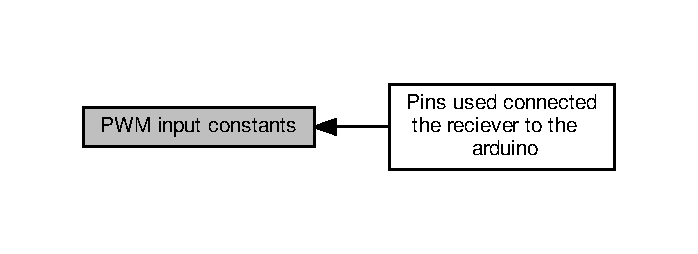
\includegraphics[width=335pt]{group__PwmInputConstants}
\end{center}
\end{figure}
\subsection*{Modules}
\begin{DoxyCompactItemize}
\item 
\hyperlink{group__RecieverPwmPins}{Pins used connected the reciever to the arduino}
\end{DoxyCompactItemize}
\subsection*{Variables}
\begin{DoxyCompactItemize}
\item 
const uint8\+\_\+t \hyperlink{group__PwmInputConstants_gae2449e7e1058591bfbfdc0901c185602}{P\+W\+M\+\_\+\+B\+U\+F\+F\+E\+R\+\_\+\+S\+I\+ZE} = 8\hypertarget{group__PwmInputConstants_gae2449e7e1058591bfbfdc0901c185602}{}\label{group__PwmInputConstants_gae2449e7e1058591bfbfdc0901c185602}

\begin{DoxyCompactList}\small\item\em P\+WM buffer size, should be a power of 2. \end{DoxyCompactList}\item 
const uint8\+\_\+t \hyperlink{group__PwmInputConstants_gafe4b1ae7ffab8edfcd8452cd3fb7bb74}{P\+W\+M\+\_\+\+I\+X\+\_\+\+M\+A\+SK} = \hyperlink{group__PwmInputConstants_gae2449e7e1058591bfbfdc0901c185602}{P\+W\+M\+\_\+\+B\+U\+F\+F\+E\+R\+\_\+\+S\+I\+ZE} -\/ 1\hypertarget{group__PwmInputConstants_gafe4b1ae7ffab8edfcd8452cd3fb7bb74}{}\label{group__PwmInputConstants_gafe4b1ae7ffab8edfcd8452cd3fb7bb74}

\begin{DoxyCompactList}\small\item\em Modulo mask for buffer. \end{DoxyCompactList}\item 
const uint8\+\_\+t \hyperlink{group__PwmInputConstants_ga89098a2ff03e736c257b322e78e7c6e3}{P\+I\+N\+\_\+\+M\+A\+SK}
\begin{DoxyCompactList}\small\item\em Pin mask used for falling edge detection. \end{DoxyCompactList}\end{DoxyCompactItemize}


\subsection{Detailed Description}
Pin number are relative pin register B (pin 8...13) 

\subsection{Variable Documentation}
\index{P\+W\+M input constants@{P\+W\+M input constants}!P\+I\+N\+\_\+\+M\+A\+SK@{P\+I\+N\+\_\+\+M\+A\+SK}}
\index{P\+I\+N\+\_\+\+M\+A\+SK@{P\+I\+N\+\_\+\+M\+A\+SK}!P\+W\+M input constants@{P\+W\+M input constants}}
\subsubsection[{\texorpdfstring{P\+I\+N\+\_\+\+M\+A\+SK}{PIN_MASK}}]{\setlength{\rightskip}{0pt plus 5cm}const uint8\+\_\+t P\+I\+N\+\_\+\+M\+A\+SK}\hypertarget{group__PwmInputConstants_ga89098a2ff03e736c257b322e78e7c6e3}{}\label{group__PwmInputConstants_ga89098a2ff03e736c257b322e78e7c6e3}
{\bfseries Initial value\+:}
\begin{DoxyCode}
= bit(\hyperlink{group__RecieverPwmPins_ga2a0f80bf9db172cf17bb4b928e861c50}{STEER\_PIN}) 
                       | bit(\hyperlink{group__RecieverPwmPins_gafee863b6234dfd9b3a4d97265e4a9a8a}{SPEED\_PIN})
                       | bit(\hyperlink{group__RecieverPwmPins_gaa1ed2fccc158e7fcb5aab8eb00e39b72}{GEAR\_PIN})
                       | bit(\hyperlink{group__RecieverPwmPins_ga91432e122cb52e765d68aed43104e478}{FDIFF\_PIN})
                       | bit(\hyperlink{group__RecieverPwmPins_ga98a9ce3925b9f576ed03843a3c6c1623}{RDIFF\_PIN})
\end{DoxyCode}


Pin mask used for falling edge detection. 



Definition at line 82 of file svea\+\_\+arduino\+\_\+src.\+h.


\hypertarget{group__RecieverPwmPins}{}\section{Pins used connected the reciever to the arduino}
\label{group__RecieverPwmPins}\index{Pins used connected the reciever to the arduino@{Pins used connected the reciever to the arduino}}
Collaboration diagram for Pins used connected the reciever to the arduino\+:\nopagebreak
\begin{figure}[H]
\begin{center}
\leavevmode
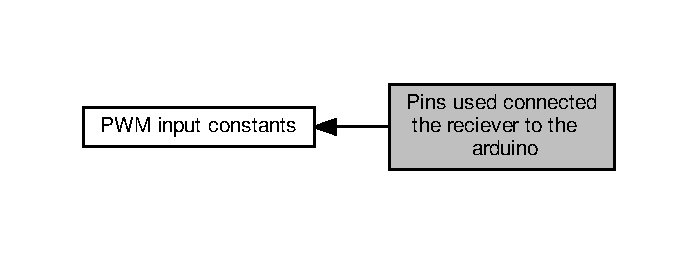
\includegraphics[width=335pt]{group__RecieverPwmPins}
\end{center}
\end{figure}
\subsection*{Variables}
\begin{DoxyCompactItemize}
\item 
const uint8\+\_\+t \hyperlink{group__RecieverPwmPins_ga2a0f80bf9db172cf17bb4b928e861c50}{S\+T\+E\+E\+R\+\_\+\+P\+IN} = 0\hypertarget{group__RecieverPwmPins_ga2a0f80bf9db172cf17bb4b928e861c50}{}\label{group__RecieverPwmPins_ga2a0f80bf9db172cf17bb4b928e861c50}

\begin{DoxyCompactList}\small\item\em D8, Steering, connect to channel 1 on the reciever. \end{DoxyCompactList}\item 
const uint8\+\_\+t \hyperlink{group__RecieverPwmPins_gafee863b6234dfd9b3a4d97265e4a9a8a}{S\+P\+E\+E\+D\+\_\+\+P\+IN} = 1\hypertarget{group__RecieverPwmPins_gafee863b6234dfd9b3a4d97265e4a9a8a}{}\label{group__RecieverPwmPins_gafee863b6234dfd9b3a4d97265e4a9a8a}

\begin{DoxyCompactList}\small\item\em D9, Velocity, connect to channel 2 on the reciever. \end{DoxyCompactList}\item 
const uint8\+\_\+t \hyperlink{group__RecieverPwmPins_gaa1ed2fccc158e7fcb5aab8eb00e39b72}{G\+E\+A\+R\+\_\+\+P\+IN} = 2\hypertarget{group__RecieverPwmPins_gaa1ed2fccc158e7fcb5aab8eb00e39b72}{}\label{group__RecieverPwmPins_gaa1ed2fccc158e7fcb5aab8eb00e39b72}

\begin{DoxyCompactList}\small\item\em D10, Transmission, connect to channel 3 on the reciever. \end{DoxyCompactList}\item 
const uint8\+\_\+t \hyperlink{group__RecieverPwmPins_ga91432e122cb52e765d68aed43104e478}{F\+D\+I\+F\+F\+\_\+\+P\+IN} = 3\hypertarget{group__RecieverPwmPins_ga91432e122cb52e765d68aed43104e478}{}\label{group__RecieverPwmPins_ga91432e122cb52e765d68aed43104e478}

\begin{DoxyCompactList}\small\item\em D11, Front differential, connect to channel 4 on the reciever. \end{DoxyCompactList}\item 
const uint8\+\_\+t \hyperlink{group__RecieverPwmPins_ga98a9ce3925b9f576ed03843a3c6c1623}{R\+D\+I\+F\+F\+\_\+\+P\+IN} = 4\hypertarget{group__RecieverPwmPins_ga98a9ce3925b9f576ed03843a3c6c1623}{}\label{group__RecieverPwmPins_ga98a9ce3925b9f576ed03843a3c6c1623}

\begin{DoxyCompactList}\small\item\em D12, Rear differential, connect to channel 5 on the reciever. \end{DoxyCompactList}\end{DoxyCompactItemize}


\subsection{Detailed Description}
Pin number are relative pin register B (pin 8...13) 
\hypertarget{group__EncoderPins}{}\section{Pins used connected the wheel encoders.}
\label{group__EncoderPins}\index{Pins used connected the wheel encoders.@{Pins used connected the wheel encoders.}}
\subsection*{Variables}
\begin{DoxyCompactItemize}
\item 
const uint8\+\_\+t \hyperlink{group__EncoderPins_ga14cc250717e67ba33ff892452b2454b7}{E\+N\+C\+O\+D\+E\+R\+\_\+\+P\+I\+N\+\_\+R} = 6\hypertarget{group__EncoderPins_ga14cc250717e67ba33ff892452b2454b7}{}\label{group__EncoderPins_ga14cc250717e67ba33ff892452b2454b7}

\begin{DoxyCompactList}\small\item\em D6, Right wheel encoder tick pin. \end{DoxyCompactList}\item 
const uint8\+\_\+t \hyperlink{group__EncoderPins_gac51556d78c19fe7342678805ccc77b57}{E\+N\+C\+O\+D\+E\+R\+\_\+\+P\+I\+N\+\_\+L} = 7\hypertarget{group__EncoderPins_gac51556d78c19fe7342678805ccc77b57}{}\label{group__EncoderPins_gac51556d78c19fe7342678805ccc77b57}

\begin{DoxyCompactList}\small\item\em D7, Left wheel encoder tick pin. \end{DoxyCompactList}\end{DoxyCompactItemize}


\subsection{Detailed Description}
Have to be in the range of P\+O\+R\+TD (pin D0 to D7) and D0 to D3 are reserved. 
\hypertarget{group__MsgBitPositions}{}\section{Bit positions used for the trans\+\_\+diff\+\_\+ctrl field in messages}
\label{group__MsgBitPositions}\index{Bit positions used for the trans\+\_\+diff\+\_\+ctrl field in messages@{Bit positions used for the trans\+\_\+diff\+\_\+ctrl field in messages}}
\subsection*{Variables}
\begin{DoxyCompactItemize}
\item 
const uint8\+\_\+t \hyperlink{group__MsgBitPositions_ga34eaead62b770ea48065591164ec9e29}{G\+E\+A\+R\+\_\+\+B\+IT} = 0\hypertarget{group__MsgBitPositions_ga34eaead62b770ea48065591164ec9e29}{}\label{group__MsgBitPositions_ga34eaead62b770ea48065591164ec9e29}

\begin{DoxyCompactList}\small\item\em Bit used for gear value (0 unlocked, 1 locked) \end{DoxyCompactList}\item 
const uint8\+\_\+t \hyperlink{group__MsgBitPositions_ga9b82b2c57fd205efb6f330b75d48c8dc}{F\+D\+I\+F\+F\+\_\+\+B\+IT} = 1\hypertarget{group__MsgBitPositions_ga9b82b2c57fd205efb6f330b75d48c8dc}{}\label{group__MsgBitPositions_ga9b82b2c57fd205efb6f330b75d48c8dc}

\begin{DoxyCompactList}\small\item\em Bit used for front differential value (0 unlocked, 1 locked) \end{DoxyCompactList}\item 
const uint8\+\_\+t \hyperlink{group__MsgBitPositions_ga4f5aa3ea23a63189068319996dc40fc5}{R\+D\+I\+F\+F\+\_\+\+B\+IT} = 2
\item 
const uint8\+\_\+t \hyperlink{group__MsgBitPositions_ga72cf872102541424c2048e61e50c0709}{A\+C\+T\+\_\+\+B\+I\+TS} \mbox{[}3\mbox{]} = \{\hyperlink{group__MsgBitPositions_ga34eaead62b770ea48065591164ec9e29}{G\+E\+A\+R\+\_\+\+B\+IT}, \hyperlink{group__MsgBitPositions_ga9b82b2c57fd205efb6f330b75d48c8dc}{F\+D\+I\+F\+F\+\_\+\+B\+IT}, \hyperlink{group__MsgBitPositions_ga4f5aa3ea23a63189068319996dc40fc5}{R\+D\+I\+F\+F\+\_\+\+B\+IT}\}\hypertarget{group__MsgBitPositions_ga72cf872102541424c2048e61e50c0709}{}\label{group__MsgBitPositions_ga72cf872102541424c2048e61e50c0709}

\begin{DoxyCompactList}\small\item\em Vector with the bit postitions in msg.\+gear\+\_\+diff in order\+: gear, front diff, rear diff. \end{DoxyCompactList}\item 
const uint8\+\_\+t \hyperlink{group__MsgBitPositions_ga9f523412ec86e2d7c6ecd3c1a49a2d9b}{E\+N\+A\+B\+L\+E\+\_\+\+G\+E\+A\+R\+C\+H\+A\+N\+G\+E\+\_\+\+B\+IT} = 3\hypertarget{group__MsgBitPositions_ga9f523412ec86e2d7c6ecd3c1a49a2d9b}{}\label{group__MsgBitPositions_ga9f523412ec86e2d7c6ecd3c1a49a2d9b}

\begin{DoxyCompactList}\small\item\em Bit indicating if the G\+E\+A\+R\+\_\+\+B\+IT value should be read from incoming messages. \end{DoxyCompactList}\item 
const uint8\+\_\+t \hyperlink{group__MsgBitPositions_ga62390c182ca2894e4370302b2ee56ed9}{E\+N\+A\+B\+L\+E\+\_\+\+F\+D\+I\+F\+C\+H\+A\+N\+G\+E\+\_\+\+B\+IT} = 4\hypertarget{group__MsgBitPositions_ga62390c182ca2894e4370302b2ee56ed9}{}\label{group__MsgBitPositions_ga62390c182ca2894e4370302b2ee56ed9}

\begin{DoxyCompactList}\small\item\em Bit indicating if the front differential values should be read from incoming messages. \end{DoxyCompactList}\item 
const uint8\+\_\+t \hyperlink{group__MsgBitPositions_gabd2bfd09673f529363f995d6ea7a94fb}{E\+N\+A\+B\+L\+E\+\_\+\+R\+D\+I\+F\+C\+H\+A\+N\+G\+E\+\_\+\+B\+IT} = 5\hypertarget{group__MsgBitPositions_gabd2bfd09673f529363f995d6ea7a94fb}{}\label{group__MsgBitPositions_gabd2bfd09673f529363f995d6ea7a94fb}

\begin{DoxyCompactList}\small\item\em Bit indicating if the rear differential values should be read from incoming messages. \end{DoxyCompactList}\item 
const uint8\+\_\+t \hyperlink{group__MsgBitPositions_gafee1df3a4ab5fca7535d372d876036ea}{E\+N\+A\+B\+L\+E\+\_\+\+A\+C\+T\+\_\+\+C\+H\+A\+N\+G\+E\+\_\+\+B\+I\+TS} \mbox{[}3\mbox{]} = \{\hyperlink{group__MsgBitPositions_ga9f523412ec86e2d7c6ecd3c1a49a2d9b}{E\+N\+A\+B\+L\+E\+\_\+\+G\+E\+A\+R\+C\+H\+A\+N\+G\+E\+\_\+\+B\+IT}, \hyperlink{group__MsgBitPositions_ga62390c182ca2894e4370302b2ee56ed9}{E\+N\+A\+B\+L\+E\+\_\+\+F\+D\+I\+F\+C\+H\+A\+N\+G\+E\+\_\+\+B\+IT}, \hyperlink{group__MsgBitPositions_gabd2bfd09673f529363f995d6ea7a94fb}{E\+N\+A\+B\+L\+E\+\_\+\+R\+D\+I\+F\+C\+H\+A\+N\+G\+E\+\_\+\+B\+IT}\}\hypertarget{group__MsgBitPositions_gafee1df3a4ab5fca7535d372d876036ea}{}\label{group__MsgBitPositions_gafee1df3a4ab5fca7535d372d876036ea}

\begin{DoxyCompactList}\small\item\em Vector with the enable change bits in order\+: gear, front diff, rear diff. \end{DoxyCompactList}\item 
const int8\+\_\+t \hyperlink{group__MsgBitPositions_ga7e9874545710fd223a9d783f83e11a62}{M\+S\+G\+\_\+\+T\+O\+\_\+\+A\+C\+T\+\_\+\+O\+FF} \mbox{[}3\mbox{]} = \{\hyperlink{group__ActuationToOutput_ga54b4e4d7476d53406564c1e9159df212}{I\+N\+P\+U\+T\+\_\+\+M\+AX}, \hyperlink{group__ActuationToOutput_ga54b4e4d7476d53406564c1e9159df212}{I\+N\+P\+U\+T\+\_\+\+M\+AX}-\/10, \hyperlink{group__ActuationToOutput_ga1f805f05ca679b7b28951bfa6659294d}{I\+N\+P\+U\+T\+\_\+\+M\+IN}+10\}\hypertarget{group__MsgBitPositions_ga7e9874545710fd223a9d783f83e11a62}{}\label{group__MsgBitPositions_ga7e9874545710fd223a9d783f83e11a62}

\begin{DoxyCompactList}\small\item\em Value that should be actuated if the corresponding bit in msg.\+gear\+\_\+diff is not set. \end{DoxyCompactList}\item 
const int8\+\_\+t \hyperlink{group__MsgBitPositions_gaf2abc78dd02137e1e3c98f381c80efc5}{M\+S\+G\+\_\+\+T\+O\+\_\+\+A\+C\+T\+\_\+\+ON} \mbox{[}3\mbox{]} = \{\hyperlink{group__ActuationToOutput_ga1f805f05ca679b7b28951bfa6659294d}{I\+N\+P\+U\+T\+\_\+\+M\+IN}, \hyperlink{group__ActuationToOutput_ga1f805f05ca679b7b28951bfa6659294d}{I\+N\+P\+U\+T\+\_\+\+M\+IN}+10, \hyperlink{group__ActuationToOutput_ga54b4e4d7476d53406564c1e9159df212}{I\+N\+P\+U\+T\+\_\+\+M\+AX}-\/10\}\hypertarget{group__MsgBitPositions_gaf2abc78dd02137e1e3c98f381c80efc5}{}\label{group__MsgBitPositions_gaf2abc78dd02137e1e3c98f381c80efc5}

\begin{DoxyCompactList}\small\item\em Value that should be actuated if the corresponding bit in msg.\+gear\+\_\+diff is not set. \end{DoxyCompactList}\end{DoxyCompactItemize}


\subsection{Detailed Description}


\subsection{Variable Documentation}
\index{Bit positions used for the trans\+\_\+diff\+\_\+ctrl field in messages@{Bit positions used for the trans\+\_\+diff\+\_\+ctrl field in messages}!R\+D\+I\+F\+F\+\_\+\+B\+IT@{R\+D\+I\+F\+F\+\_\+\+B\+IT}}
\index{R\+D\+I\+F\+F\+\_\+\+B\+IT@{R\+D\+I\+F\+F\+\_\+\+B\+IT}!Bit positions used for the trans\+\_\+diff\+\_\+ctrl field in messages@{Bit positions used for the trans\+\_\+diff\+\_\+ctrl field in messages}}
\subsubsection[{\texorpdfstring{R\+D\+I\+F\+F\+\_\+\+B\+IT}{RDIFF_BIT}}]{\setlength{\rightskip}{0pt plus 5cm}const uint8\+\_\+t R\+D\+I\+F\+F\+\_\+\+B\+IT = 2}\hypertarget{group__MsgBitPositions_ga4f5aa3ea23a63189068319996dc40fc5}{}\label{group__MsgBitPositions_ga4f5aa3ea23a63189068319996dc40fc5}
Bit used for rear differential value (0 unlocked, 1 locked) 

Definition at line 118 of file svea\+\_\+arduino\+\_\+src.\+h.


\hypertarget{group__ActuationValueStorage}{}\section{Actuation value storage}
\label{group__ActuationValueStorage}\index{Actuation value storage@{Actuation value storage}}
\subsection*{Variables}
\begin{DoxyCompactItemize}
\item 
int8\+\_\+t \hyperlink{group__ActuationValueStorage_ga7c78ea1be4ba9168380940fe5fdb889f}{S\+W\+\_\+\+A\+C\+T\+U\+A\+T\+I\+ON} \mbox{[}5\mbox{]} = \{0,0,\hyperlink{group__MsgBitPositions_ga7e9874545710fd223a9d783f83e11a62}{M\+S\+G\+\_\+\+T\+O\+\_\+\+A\+C\+T\+\_\+\+O\+FF}\mbox{[}0\mbox{]},\hyperlink{group__MsgBitPositions_ga7e9874545710fd223a9d783f83e11a62}{M\+S\+G\+\_\+\+T\+O\+\_\+\+A\+C\+T\+\_\+\+O\+FF}\mbox{[}1\mbox{]},\hyperlink{group__MsgBitPositions_ga7e9874545710fd223a9d783f83e11a62}{M\+S\+G\+\_\+\+T\+O\+\_\+\+A\+C\+T\+\_\+\+O\+FF}\mbox{[}2\mbox{]}\}\hypertarget{group__ActuationValueStorage_ga7c78ea1be4ba9168380940fe5fdb889f}{}\label{group__ActuationValueStorage_ga7c78ea1be4ba9168380940fe5fdb889f}

\begin{DoxyCompactList}\small\item\em Actuation values sent from the computer. \end{DoxyCompactList}\item 
int8\+\_\+t \hyperlink{group__ActuationValueStorage_gaa62470a230859dd30f46b50aa6c0536e}{R\+E\+M\+\_\+\+A\+C\+T\+U\+A\+T\+I\+ON} \mbox{[}5\mbox{]} = \{0,0,\hyperlink{group__MsgBitPositions_ga7e9874545710fd223a9d783f83e11a62}{M\+S\+G\+\_\+\+T\+O\+\_\+\+A\+C\+T\+\_\+\+O\+FF}\mbox{[}0\mbox{]},\hyperlink{group__MsgBitPositions_ga7e9874545710fd223a9d783f83e11a62}{M\+S\+G\+\_\+\+T\+O\+\_\+\+A\+C\+T\+\_\+\+O\+FF}\mbox{[}1\mbox{]},\hyperlink{group__MsgBitPositions_ga7e9874545710fd223a9d783f83e11a62}{M\+S\+G\+\_\+\+T\+O\+\_\+\+A\+C\+T\+\_\+\+O\+FF}\mbox{[}2\mbox{]}\}\hypertarget{group__ActuationValueStorage_gaa62470a230859dd30f46b50aa6c0536e}{}\label{group__ActuationValueStorage_gaa62470a230859dd30f46b50aa6c0536e}

\begin{DoxyCompactList}\small\item\em Actuation values sent from the remote. \end{DoxyCompactList}\item 
const int8\+\_\+t \hyperlink{group__ActuationValueStorage_ga39e6648fcb502c3da718d80b661974ae}{I\+D\+L\+E\+\_\+\+A\+C\+T\+U\+A\+T\+I\+ON} \mbox{[}5\mbox{]} = \{0,0,0,\hyperlink{group__MsgBitPositions_ga7e9874545710fd223a9d783f83e11a62}{M\+S\+G\+\_\+\+T\+O\+\_\+\+A\+C\+T\+\_\+\+O\+FF}\mbox{[}1\mbox{]},\hyperlink{group__MsgBitPositions_ga7e9874545710fd223a9d783f83e11a62}{M\+S\+G\+\_\+\+T\+O\+\_\+\+A\+C\+T\+\_\+\+O\+FF}\mbox{[}2\mbox{]}\}\hypertarget{group__ActuationValueStorage_ga39e6648fcb502c3da718d80b661974ae}{}\label{group__ActuationValueStorage_ga39e6648fcb502c3da718d80b661974ae}

\begin{DoxyCompactList}\small\item\em Actuation values sent when both the remote and the computer are idle. \end{DoxyCompactList}\end{DoxyCompactItemize}


\subsection{Detailed Description}
The order is Steering, velocity, gear, front differential, rear differential 
\hypertarget{group__PwmMeasurtement}{}\section{Reciever pwm duty cycle measurement variables}
\label{group__PwmMeasurtement}\index{Reciever pwm duty cycle measurement variables@{Reciever pwm duty cycle measurement variables}}
\subsection*{Variables}
\begin{DoxyCompactItemize}
\item 
volatile long \hyperlink{group__PwmMeasurtement_gaeb758acd90cce2a48375254eb9c2d843}{P\+W\+M\+\_\+\+H\+I\+G\+H\+\_\+\+T\+I\+ME}
\item 
volatile bool \hyperlink{group__PwmMeasurtement_ga1ca1be2c986a00d6a79e5d7d5ab1313c}{H\+I\+G\+H\+\_\+\+R\+E\+C\+I\+E\+V\+ED} = false\hypertarget{group__PwmMeasurtement_ga1ca1be2c986a00d6a79e5d7d5ab1313c}{}\label{group__PwmMeasurtement_ga1ca1be2c986a00d6a79e5d7d5ab1313c}

\begin{DoxyCompactList}\small\item\em True if a rising edge has been observed since the latest values was sent to R\+OS. \end{DoxyCompactList}\item 
volatile uint8\+\_\+t \hyperlink{group__PwmMeasurtement_ga3f84f08978073d634ef59d44eba3c32a}{I\+N\+T\+\_\+\+P\+I\+N\+\_\+\+S\+T\+A\+T\+US} = 0\hypertarget{group__PwmMeasurtement_ga3f84f08978073d634ef59d44eba3c32a}{}\label{group__PwmMeasurtement_ga3f84f08978073d634ef59d44eba3c32a}

\begin{DoxyCompactList}\small\item\em Indicates which pins that are still high since the last rising edge. \end{DoxyCompactList}\item 
volatile unsigned long \hyperlink{group__PwmMeasurtement_ga1980b7b5ba1ceabb0b5c60c9da70164e}{P\+W\+M\+\_\+\+T\+\_\+\+B\+U\+F\+F\+ER} \mbox{[}\hyperlink{group__PwmInputConstants_gae2449e7e1058591bfbfdc0901c185602}{P\+W\+M\+\_\+\+B\+U\+F\+F\+E\+R\+\_\+\+S\+I\+ZE}\mbox{]}\hypertarget{group__PwmMeasurtement_ga1980b7b5ba1ceabb0b5c60c9da70164e}{}\label{group__PwmMeasurtement_ga1980b7b5ba1ceabb0b5c60c9da70164e}

\begin{DoxyCompactList}\small\item\em Falling edge interrupt time buffer. \end{DoxyCompactList}\item 
volatile uint8\+\_\+t \hyperlink{group__PwmMeasurtement_gaed4f8ecf3e1ca2d8bfa8904a43729f57}{P\+W\+M\+\_\+\+S\+\_\+\+B\+U\+F\+F\+ER} \mbox{[}\hyperlink{group__PwmInputConstants_gae2449e7e1058591bfbfdc0901c185602}{P\+W\+M\+\_\+\+B\+U\+F\+F\+E\+R\+\_\+\+S\+I\+ZE}\mbox{]}\hypertarget{group__PwmMeasurtement_gaed4f8ecf3e1ca2d8bfa8904a43729f57}{}\label{group__PwmMeasurtement_gaed4f8ecf3e1ca2d8bfa8904a43729f57}

\begin{DoxyCompactList}\small\item\em Falling edge interrupt pin readig buffer. \end{DoxyCompactList}\item 
volatile uint8\+\_\+t \hyperlink{group__PwmMeasurtement_ga240562bcf38322f5e5fe4498c0884a79}{P\+W\+M\+\_\+\+B\+U\+F\+F\+E\+R\+\_\+\+W\+\_\+\+IX} = 0\hypertarget{group__PwmMeasurtement_ga240562bcf38322f5e5fe4498c0884a79}{}\label{group__PwmMeasurtement_ga240562bcf38322f5e5fe4498c0884a79}

\begin{DoxyCompactList}\small\item\em Pwm buffers read index. \end{DoxyCompactList}\item 
volatile uint8\+\_\+t \hyperlink{group__PwmMeasurtement_gac0879dcb58dda890aceef95b7f4bc793}{P\+W\+M\+\_\+\+B\+U\+F\+F\+E\+R\+\_\+\+R\+\_\+\+IX} = 0\hypertarget{group__PwmMeasurtement_gac0879dcb58dda890aceef95b7f4bc793}{}\label{group__PwmMeasurtement_gac0879dcb58dda890aceef95b7f4bc793}

\begin{DoxyCompactList}\small\item\em Pwm buffers write index. \end{DoxyCompactList}\end{DoxyCompactItemize}


\subsection{Detailed Description}


\subsection{Variable Documentation}
\index{Reciever pwm duty cycle measurement variables@{Reciever pwm duty cycle measurement variables}!P\+W\+M\+\_\+\+H\+I\+G\+H\+\_\+\+T\+I\+ME@{P\+W\+M\+\_\+\+H\+I\+G\+H\+\_\+\+T\+I\+ME}}
\index{P\+W\+M\+\_\+\+H\+I\+G\+H\+\_\+\+T\+I\+ME@{P\+W\+M\+\_\+\+H\+I\+G\+H\+\_\+\+T\+I\+ME}!Reciever pwm duty cycle measurement variables@{Reciever pwm duty cycle measurement variables}}
\subsubsection[{\texorpdfstring{P\+W\+M\+\_\+\+H\+I\+G\+H\+\_\+\+T\+I\+ME}{PWM_HIGH_TIME}}]{\setlength{\rightskip}{0pt plus 5cm}volatile long P\+W\+M\+\_\+\+H\+I\+G\+H\+\_\+\+T\+I\+ME}\hypertarget{group__PwmMeasurtement_gaeb758acd90cce2a48375254eb9c2d843}{}\label{group__PwmMeasurtement_gaeb758acd90cce2a48375254eb9c2d843}
Time of the last rising edge in micro seconds 

Definition at line 164 of file svea\+\_\+arduino\+\_\+src.\+h.


\hypertarget{group__EncoderVariables}{}\section{Wheel encoder variables}
\label{group__EncoderVariables}\index{Wheel encoder variables@{Wheel encoder variables}}
\subsection*{Variables}
\begin{DoxyCompactItemize}
\item 
uint8\+\_\+t \hyperlink{group__EncoderVariables_ga63bd10c23b8e1e359ccc54b26ddccf2b}{R\+I\+G\+H\+T\+\_\+\+T\+I\+C\+K\+\_\+\+C\+O\+U\+NT} = 0\hypertarget{group__EncoderVariables_ga63bd10c23b8e1e359ccc54b26ddccf2b}{}\label{group__EncoderVariables_ga63bd10c23b8e1e359ccc54b26ddccf2b}

\begin{DoxyCompactList}\small\item\em Right wheel tick count. \end{DoxyCompactList}\item 
uint8\+\_\+t \hyperlink{group__EncoderVariables_ga7b675fdfa3a53486da47f929c42ef4a8}{L\+E\+F\+T\+\_\+\+T\+I\+C\+K\+\_\+\+C\+O\+U\+NT} = 0\hypertarget{group__EncoderVariables_ga7b675fdfa3a53486da47f929c42ef4a8}{}\label{group__EncoderVariables_ga7b675fdfa3a53486da47f929c42ef4a8}

\begin{DoxyCompactList}\small\item\em left wheel tick count \end{DoxyCompactList}\end{DoxyCompactItemize}


\subsection{Detailed Description}

\hypertarget{group__StatusVariables}{}\section{Status variables}
\label{group__StatusVariables}\index{Status variables@{Status variables}}
\subsection*{Variables}
\begin{DoxyCompactItemize}
\item 
unsigned long \hyperlink{group__StatusVariables_ga82efae9ec88cdde7eaa3cd149aa5756c}{S\+W\+\_\+\+T\+\_\+\+R\+E\+C\+I\+E\+V\+ED} =millis()\hypertarget{group__StatusVariables_ga82efae9ec88cdde7eaa3cd149aa5756c}{}\label{group__StatusVariables_ga82efae9ec88cdde7eaa3cd149aa5756c}

\begin{DoxyCompactList}\small\item\em Time when last message was recieved from the computer. \end{DoxyCompactList}\item 
bool \hyperlink{group__StatusVariables_ga1dc5fbe81aa54db10c814d5ff7adba6f}{R\+E\+M\+\_\+\+I\+D\+LE} = true\hypertarget{group__StatusVariables_ga1dc5fbe81aa54db10c814d5ff7adba6f}{}\label{group__StatusVariables_ga1dc5fbe81aa54db10c814d5ff7adba6f}

\begin{DoxyCompactList}\small\item\em True if the remote is considered idle. \end{DoxyCompactList}\item 
bool \hyperlink{group__StatusVariables_gae31e17311163c382d2de940091954419}{R\+E\+M\+\_\+\+O\+V\+E\+R\+R\+I\+DE} = false\hypertarget{group__StatusVariables_gae31e17311163c382d2de940091954419}{}\label{group__StatusVariables_gae31e17311163c382d2de940091954419}

\begin{DoxyCompactList}\small\item\em True if the remote should override computer inputs. \end{DoxyCompactList}\item 
bool \hyperlink{group__StatusVariables_ga5f2f8cd3c1e83a4aac8976d9dbb71e4b}{S\+W\+\_\+\+I\+D\+LE} = true\hypertarget{group__StatusVariables_ga5f2f8cd3c1e83a4aac8976d9dbb71e4b}{}\label{group__StatusVariables_ga5f2f8cd3c1e83a4aac8976d9dbb71e4b}

\begin{DoxyCompactList}\small\item\em True if the computer is considered idle. \end{DoxyCompactList}\end{DoxyCompactItemize}


\subsection{Detailed Description}

\hypertarget{group__ROSSetup}{}\section{Variables used by R\+OS}
\label{group__ROSSetup}\index{Variables used by R\+OS@{Variables used by R\+OS}}
\subsection*{Functions}
\begin{DoxyCompactItemize}
\item 
ros\+::\+Publisher \hyperlink{group__ROSSetup_ga93b3bd1d04d33169e1a28258a8b07af7}{remote\+\_\+pub} (\char`\"{}/lli/remote\char`\"{},\&M\+S\+G\+\_\+\+R\+E\+M\+O\+TE)\hypertarget{group__ROSSetup_ga93b3bd1d04d33169e1a28258a8b07af7}{}\label{group__ROSSetup_ga93b3bd1d04d33169e1a28258a8b07af7}

\begin{DoxyCompactList}\small\item\em Remote message publisher. \end{DoxyCompactList}\item 
ros\+::\+Publisher \hyperlink{group__ROSSetup_ga3053db74e7b16c6af3d7eda6d8b0c83c}{ctrl\+\_\+actuated\+\_\+pub} (\char`\"{}/lli/ctrl\+\_\+actuated\char`\"{},\&M\+S\+G\+\_\+\+A\+C\+T\+U\+A\+T\+ED)\hypertarget{group__ROSSetup_ga3053db74e7b16c6af3d7eda6d8b0c83c}{}\label{group__ROSSetup_ga3053db74e7b16c6af3d7eda6d8b0c83c}

\begin{DoxyCompactList}\small\item\em Actuated control message publisher. \end{DoxyCompactList}\item 
ros\+::\+Publisher \hyperlink{group__ROSSetup_gae33f55282b004e6f50e44ec7df40c321}{encoder\+\_\+pub} (\char`\"{}/lli/encoder\char`\"{},\&M\+S\+G\+\_\+\+E\+N\+C\+O\+D\+ER)\hypertarget{group__ROSSetup_gae33f55282b004e6f50e44ec7df40c321}{}\label{group__ROSSetup_gae33f55282b004e6f50e44ec7df40c321}

\begin{DoxyCompactList}\small\item\em Encoder reading publisher. \end{DoxyCompactList}\item 
ros\+::\+Subscriber$<$ \hyperlink{svea__arduino__src_8h_a397644608f772ef60685f6a938f43ea1}{lli\+\_\+ctrl\+\_\+in} $>$ \hyperlink{group__ROSSetup_ga9fcbca83450aa2c5c64cde1a0e0557c5}{ctrl\+\_\+request} (\char`\"{}/lli/ctrl\+\_\+request\char`\"{},\&cb\+\_\+ctrl\+\_\+request)\hypertarget{group__ROSSetup_ga9fcbca83450aa2c5c64cde1a0e0557c5}{}\label{group__ROSSetup_ga9fcbca83450aa2c5c64cde1a0e0557c5}

\begin{DoxyCompactList}\small\item\em Controll request subscriber. \end{DoxyCompactList}\end{DoxyCompactItemize}
\subsection*{Variables}
\begin{DoxyCompactItemize}
\item 
ros\+::\+Node\+Handle\+\_\+$<$ Arduino\+Hardware, 1, 3, 100, 100 $>$ \hyperlink{group__ROSSetup_ga9518748567d9dc49cb5d062ae16eccac}{nh}\hypertarget{group__ROSSetup_ga9518748567d9dc49cb5d062ae16eccac}{}\label{group__ROSSetup_ga9518748567d9dc49cb5d062ae16eccac}

\begin{DoxyCompactList}\small\item\em Node\+Handle class definitions. \end{DoxyCompactList}\item 
\hyperlink{svea__arduino__src_8h_a6b033df4aed2c02e82dc2962f73c2ccb}{lli\+\_\+ctrl\+\_\+out} \hyperlink{group__ROSSetup_gad1e4ff3dbb3ddc9a6fadfcc80b6b6b20}{M\+S\+G\+\_\+\+R\+E\+M\+O\+TE}\hypertarget{group__ROSSetup_gad1e4ff3dbb3ddc9a6fadfcc80b6b6b20}{}\label{group__ROSSetup_gad1e4ff3dbb3ddc9a6fadfcc80b6b6b20}

\begin{DoxyCompactList}\small\item\em Message used for sending the remote signals. \end{DoxyCompactList}\item 
\hyperlink{svea__arduino__src_8h_a6b033df4aed2c02e82dc2962f73c2ccb}{lli\+\_\+ctrl\+\_\+out} \hyperlink{group__ROSSetup_ga7b886027c8fb98155a2757bc5be08615}{M\+S\+G\+\_\+\+A\+C\+T\+U\+A\+T\+ED}\hypertarget{group__ROSSetup_ga7b886027c8fb98155a2757bc5be08615}{}\label{group__ROSSetup_ga7b886027c8fb98155a2757bc5be08615}

\begin{DoxyCompactList}\small\item\em Message sending actuated messages. \end{DoxyCompactList}\item 
lli\+\_\+encoder \hyperlink{group__ROSSetup_ga46e4ead0cae634e475c6606dd97cc393}{M\+S\+G\+\_\+\+E\+N\+C\+O\+D\+ER}\hypertarget{group__ROSSetup_ga46e4ead0cae634e475c6606dd97cc393}{}\label{group__ROSSetup_ga46e4ead0cae634e475c6606dd97cc393}

\begin{DoxyCompactList}\small\item\em Message used for outgoing wheel encoder messages. \end{DoxyCompactList}\end{DoxyCompactItemize}


\subsection{Detailed Description}

\chapter{File Documentation}
\hypertarget{settings_8h}{}\section{/home/nvidia/starter\+\_\+ws/src/svea\+\_\+starter/src/svea\+\_\+arduino/svea\+\_\+arduino\+\_\+src/settings.h File Reference}
\label{settings_8h}\index{/home/nvidia/starter\+\_\+ws/src/svea\+\_\+starter/src/svea\+\_\+arduino/svea\+\_\+arduino\+\_\+src/settings.\+h@{/home/nvidia/starter\+\_\+ws/src/svea\+\_\+starter/src/svea\+\_\+arduino/svea\+\_\+arduino\+\_\+src/settings.\+h}}
This graph shows which files directly or indirectly include this file\+:
\nopagebreak
\begin{figure}[H]
\begin{center}
\leavevmode
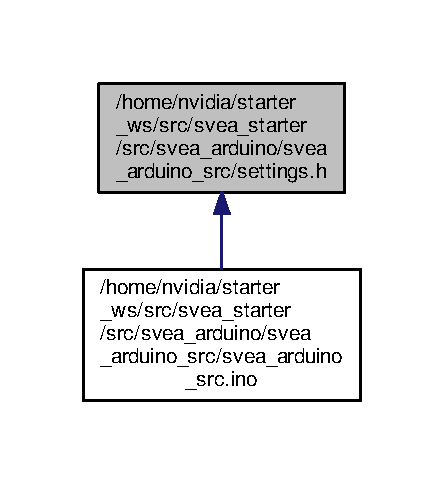
\includegraphics[width=213pt]{settings_8h__dep__incl}
\end{center}
\end{figure}
\subsection*{Variables}
\begin{DoxyCompactItemize}
\item 
const unsigned long \hyperlink{settings_8h_a829aef1874b17a2461fa716392fdab4e}{E\+N\+C\+O\+D\+E\+R\+\_\+\+S\+A\+M\+P\+L\+E\+\_\+\+I\+N\+T\+E\+R\+V\+AL} = 25000\hypertarget{settings_8h_a829aef1874b17a2461fa716392fdab4e}{}\label{settings_8h_a829aef1874b17a2461fa716392fdab4e}

\begin{DoxyCompactList}\small\item\em Sampling interval for the wheel encoders in micro seconds. \end{DoxyCompactList}\item 
const uint32\+\_\+t \hyperlink{settings_8h_af36c84a19930ad4097e8b14e0b689bee}{S\+E\+R\+I\+A\+L\+\_\+\+B\+A\+U\+D\+\_\+\+R\+A\+TE} = 250000\hypertarget{settings_8h_af36c84a19930ad4097e8b14e0b689bee}{}\label{settings_8h_af36c84a19930ad4097e8b14e0b689bee}

\begin{DoxyCompactList}\small\item\em Baud rate for serial transmisions. \end{DoxyCompactList}\item 
const uint32\+\_\+t \hyperlink{settings_8h_a95ca7fd95f43bac99d8d90b604cae239}{I2\+C\+\_\+\+F\+R\+E\+Q\+U\+E\+N\+CY} = 400000\hypertarget{settings_8h_a95ca7fd95f43bac99d8d90b604cae239}{}\label{settings_8h_a95ca7fd95f43bac99d8d90b604cae239}

\begin{DoxyCompactList}\small\item\em Baud rate for i2c transmisions. \end{DoxyCompactList}\item 
const uint8\+\_\+t \hyperlink{settings_8h_a81d1b4d200caa7d8d9694709e96f1074}{P\+W\+M\+\_\+\+R\+E\+M\+\_\+\+I\+D\+L\+E\+\_\+\+D\+E\+T\+E\+CT} = 200
\begin{DoxyCompactList}\small\item\em Duration (us) that decides when the remote should register as idle If the registred pwm singal on channel 5 from the reciever is S\+H\+O\+R\+T\+ER than this value (in microseconds), the remote is considered to be disconnected. \end{DoxyCompactList}\item 
const int8\+\_\+t {\bfseries S\+T\+E\+E\+R\+I\+N\+G\+\_\+\+C\+L\+O\+C\+K\+W\+I\+SE} = 1\hypertarget{settings_8h_abfeeb33d1dc13e229eb6fcf37f85eea8}{}\label{settings_8h_abfeeb33d1dc13e229eb6fcf37f85eea8}

\item 
const int8\+\_\+t {\bfseries S\+T\+E\+E\+R\+I\+N\+G\+\_\+\+C\+O\+U\+N\+T\+E\+R\+C\+L\+O\+C\+K\+W\+I\+SE} = -\/1\hypertarget{settings_8h_ae3591610cae2ebcf5cac82a1599c8331}{}\label{settings_8h_ae3591610cae2ebcf5cac82a1599c8331}

\item 
const int8\+\_\+t \hyperlink{settings_8h_aa8271e75d967694eef083d4a879df10f}{S\+T\+E\+E\+R\+I\+N\+G\+\_\+\+D\+I\+R\+E\+C\+T\+I\+ON} = S\+T\+E\+E\+R\+I\+N\+G\+\_\+\+C\+O\+U\+N\+T\+E\+R\+C\+L\+O\+C\+K\+W\+I\+SE\hypertarget{settings_8h_aa8271e75d967694eef083d4a879df10f}{}\label{settings_8h_aa8271e75d967694eef083d4a879df10f}

\begin{DoxyCompactList}\small\item\em Sets the steering direction that is sent and recieved from R\+OS. \end{DoxyCompactList}\item 
const uint16\+\_\+t \hyperlink{settings_8h_a4a6f8d13a634c4fbb69e18bb905c175c}{G\+E\+A\+R\+\_\+\+T\+I\+M\+E\+\_\+\+L\+I\+M\+IT} = 500\hypertarget{settings_8h_a4a6f8d13a634c4fbb69e18bb905c175c}{}\label{settings_8h_a4a6f8d13a634c4fbb69e18bb905c175c}

\begin{DoxyCompactList}\small\item\em $<$ Minimum duration (ms) between gear changes, not used \end{DoxyCompactList}\item 
const int8\+\_\+t \hyperlink{settings_8h_a8f059a42c098816d4ccebaf48add0a4a}{D\+E\+A\+D\+\_\+\+Z\+O\+NE} = 2\hypertarget{settings_8h_a8f059a42c098816d4ccebaf48add0a4a}{}\label{settings_8h_a8f059a42c098816d4ccebaf48add0a4a}

\begin{DoxyCompactList}\small\item\em Deadzone (actuation value) for actuation signals. \end{DoxyCompactList}\end{DoxyCompactItemize}
{\bf }\par
\begin{DoxyCompactItemize}
\item 
const unsigned long \hyperlink{settings_8h_afd89c92d45b41bbf8a5738ef08258106}{I\+N\+T\+E\+R\+R\+U\+P\+T\+\_\+\+D\+E\+B\+O\+U\+N\+C\+E\+\_\+\+L\+I\+M\+IT} = 2200\hypertarget{settings_8h_afd89c92d45b41bbf8a5738ef08258106}{}\label{settings_8h_afd89c92d45b41bbf8a5738ef08258106}

\begin{DoxyCompactList}\small\item\em Time in micro seconds between the detection of a pwm signal and until the dinformation is sent to R\+OS. \end{DoxyCompactList}\item 
const unsigned long \hyperlink{settings_8h_a2bc693b7f285edca340c24386beb9762}{P\+W\+M\+\_\+\+L\+O\+W\+\_\+\+L\+I\+M\+IT} = 1006\hypertarget{settings_8h_a2bc693b7f285edca340c24386beb9762}{}\label{settings_8h_a2bc693b7f285edca340c24386beb9762}

\begin{DoxyCompactList}\small\item\em Desired minimum duty cycle for the pwm board (micro seconds) \end{DoxyCompactList}\item 
const unsigned long \hyperlink{settings_8h_a0d12f57b82a32df273dc950f1e1a81f0}{P\+W\+M\+\_\+\+H\+I\+G\+H\+\_\+\+L\+I\+M\+IT} = 2000\hypertarget{settings_8h_a0d12f57b82a32df273dc950f1e1a81f0}{}\label{settings_8h_a0d12f57b82a32df273dc950f1e1a81f0}

\begin{DoxyCompactList}\small\item\em Desired maximum duty cycle for the pwm board (micro seconds) \end{DoxyCompactList}\end{DoxyCompactItemize}



\subsection{Variable Documentation}
\index{settings.\+h@{settings.\+h}!P\+W\+M\+\_\+\+R\+E\+M\+\_\+\+I\+D\+L\+E\+\_\+\+D\+E\+T\+E\+CT@{P\+W\+M\+\_\+\+R\+E\+M\+\_\+\+I\+D\+L\+E\+\_\+\+D\+E\+T\+E\+CT}}
\index{P\+W\+M\+\_\+\+R\+E\+M\+\_\+\+I\+D\+L\+E\+\_\+\+D\+E\+T\+E\+CT@{P\+W\+M\+\_\+\+R\+E\+M\+\_\+\+I\+D\+L\+E\+\_\+\+D\+E\+T\+E\+CT}!settings.\+h@{settings.\+h}}
\subsubsection[{\texorpdfstring{P\+W\+M\+\_\+\+R\+E\+M\+\_\+\+I\+D\+L\+E\+\_\+\+D\+E\+T\+E\+CT}{PWM_REM_IDLE_DETECT}}]{\setlength{\rightskip}{0pt plus 5cm}const uint8\+\_\+t P\+W\+M\+\_\+\+R\+E\+M\+\_\+\+I\+D\+L\+E\+\_\+\+D\+E\+T\+E\+CT = 200}\hypertarget{settings_8h_a81d1b4d200caa7d8d9694709e96f1074}{}\label{settings_8h_a81d1b4d200caa7d8d9694709e96f1074}


Duration (us) that decides when the remote should register as idle If the registred pwm singal on channel 5 from the reciever is S\+H\+O\+R\+T\+ER than this value (in microseconds), the remote is considered to be disconnected. 

The reciever will still send neutral steering and velocity even if the remote is of, but channel 4 and 5 (used for differentials) turns of completely. When the remote is connected again it will take approxiamtely 7 seconds until the reciever starts sending on channel 5 again, and the remote can be used again. 

Definition at line 20 of file settings.\+h.


\hypertarget{svea__arduino__src_8h}{}\section{/home/nvidia/starter\+\_\+ws/src/svea\+\_\+starter/src/svea\+\_\+arduino/svea\+\_\+arduino\+\_\+src/svea\+\_\+arduino\+\_\+src.h File Reference}
\label{svea__arduino__src_8h}\index{/home/nvidia/starter\+\_\+ws/src/svea\+\_\+starter/src/svea\+\_\+arduino/svea\+\_\+arduino\+\_\+src/svea\+\_\+arduino\+\_\+src.\+h@{/home/nvidia/starter\+\_\+ws/src/svea\+\_\+starter/src/svea\+\_\+arduino/svea\+\_\+arduino\+\_\+src/svea\+\_\+arduino\+\_\+src.\+h}}
This graph shows which files directly or indirectly include this file\+:
\nopagebreak
\begin{figure}[H]
\begin{center}
\leavevmode
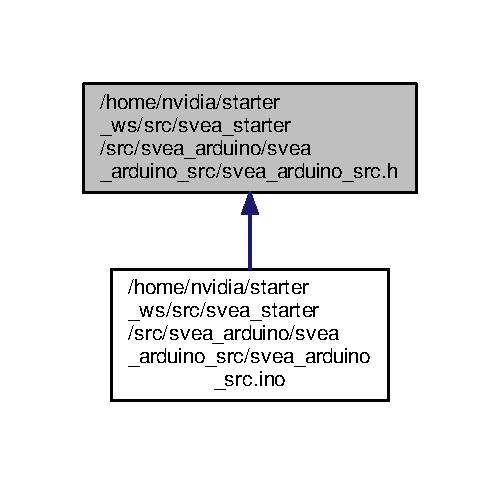
\includegraphics[width=240pt]{svea__arduino__src_8h__dep__incl}
\end{center}
\end{figure}
\subsection*{Macros}
\begin{DoxyCompactItemize}
\item 
\#define \hyperlink{svea__arduino__src_8h_aac8ead540fcc9a26a2dac8912f865e3f}{D\+U\+R\+A\+T\+I\+O\+N\+\_\+\+D\+E\+B\+UG}~0\hypertarget{svea__arduino__src_8h_aac8ead540fcc9a26a2dac8912f865e3f}{}\label{svea__arduino__src_8h_aac8ead540fcc9a26a2dac8912f865e3f}

\begin{DoxyCompactList}\small\item\em Enable/\+Disable reciever duration readouts over serial port. \end{DoxyCompactList}\end{DoxyCompactItemize}
\subsection*{Typedefs}
\begin{DoxyCompactItemize}
\item 
typedef svea\+\_\+arduino\+::lli\+\_\+ctrl \hyperlink{svea__arduino__src_8h_a397644608f772ef60685f6a938f43ea1}{lli\+\_\+ctrl\+\_\+in}\hypertarget{svea__arduino__src_8h_a397644608f772ef60685f6a938f43ea1}{}\label{svea__arduino__src_8h_a397644608f772ef60685f6a938f43ea1}

\begin{DoxyCompactList}\small\item\em Message type for incomming messages. \end{DoxyCompactList}\item 
typedef svea\+\_\+arduino\+::lli\+\_\+ctrl \hyperlink{svea__arduino__src_8h_a6b033df4aed2c02e82dc2962f73c2ccb}{lli\+\_\+ctrl\+\_\+out}\hypertarget{svea__arduino__src_8h_a6b033df4aed2c02e82dc2962f73c2ccb}{}\label{svea__arduino__src_8h_a6b033df4aed2c02e82dc2962f73c2ccb}

\begin{DoxyCompactList}\small\item\em Message type for outgoing messages\textquotesingle{}. \end{DoxyCompactList}\item 
typedef svea\+\_\+arduino\+::lli\+\_\+encoder {\bfseries lli\+\_\+encoder}\hypertarget{svea__arduino__src_8h_a79e81db84cbb5c8bfe665f4edf28a120}{}\label{svea__arduino__src_8h_a79e81db84cbb5c8bfe665f4edf28a120}

\end{DoxyCompactItemize}
\subsection*{Functions}
\begin{DoxyCompactItemize}
\item 
void \hyperlink{svea__arduino__src_8h_adab070eb39b45b4c79b5d7e3cafa9514}{set\+\_\+pwm\+\_\+driver} (uint8\+\_\+t channel, int8\+\_\+t in\+\_\+value)
\begin{DoxyCompactList}\small\item\em Set actuation P\+WM convert a 8 bit actuation value to a pwm signal and send it to the pwm board. The value gets scaled to a duration that suits the servos (approximately 1 to 2 milli seconds). The scalling uses frequency measurements from pin 10 on the pwm board. \end{DoxyCompactList}\item 
void \hyperlink{svea__arduino__src_8h_aa5545eb35f187e5fd11a483a265bed7b}{actuate} (const int8\+\_\+t actuation\+\_\+values\mbox{[}$\,$\mbox{]})
\begin{DoxyCompactList}\small\item\em Send settings to the pwm board through \hyperlink{svea__arduino__src_8ino_adab070eb39b45b4c79b5d7e3cafa9514}{set\+\_\+pwm\+\_\+driver()} \end{DoxyCompactList}\item 
uint8\+\_\+t \hyperlink{svea__arduino__src_8h_ad7d57085af575cbb5dc21e523f3a3321}{set\+\_\+actuated\+\_\+code} ()\hypertarget{svea__arduino__src_8h_ad7d57085af575cbb5dc21e523f3a3321}{}\label{svea__arduino__src_8h_ad7d57085af575cbb5dc21e523f3a3321}

\begin{DoxyCompactList}\small\item\em set the control code in messages sent to the computer \end{DoxyCompactList}\item 
void \hyperlink{svea__arduino__src_8h_ae79b6def446edd5a233efe74bc1f2a7b}{cb\+\_\+ctrl\+\_\+request} (const \hyperlink{svea__arduino__src_8h_a397644608f772ef60685f6a938f43ea1}{lli\+\_\+ctrl\+\_\+in} \&data)
\begin{DoxyCompactList}\small\item\em Callback function for control requests from R\+OS Interprets the message and sends the values to the pwm board through \hyperlink{svea__arduino__src_8ino_aa5545eb35f187e5fd11a483a265bed7b}{actuate()}. \end{DoxyCompactList}\item 
int8\+\_\+t \hyperlink{svea__arduino__src_8h_a1c4a5154127fe3f9963eb968b0714b90}{pwm\+\_\+to\+\_\+actuation} (unsigned long duration)
\item 
void \hyperlink{svea__arduino__src_8h_a2948125fe6592c36c5c0e641478e2db0}{pwm\+Event} ()\hypertarget{svea__arduino__src_8h_a2948125fe6592c36c5c0e641478e2db0}{}\label{svea__arduino__src_8h_a2948125fe6592c36c5c0e641478e2db0}

\begin{DoxyCompactList}\small\item\em Called when a pwm signal from the remote has been recieved Takes the actuation values from the remote and sends them to R\+OS. The frequency of the R\+OS messages is around 100 Hz, based on the frequency of the reciever. If the computer is not sending any signals or the \hyperlink{group__StatusVariables_gae31e17311163c382d2de940091954419}{R\+E\+M\+\_\+\+O\+V\+E\+R\+R\+I\+DE} flag is set (by pushing the deifferential switch to the formost position) the actuation values will also be sent to the pwm board through \hyperlink{svea__arduino__src_8ino_aa5545eb35f187e5fd11a483a265bed7b}{actuate()}. \end{DoxyCompactList}\item 
void \hyperlink{svea__arduino__src_8h_af99fa97e441e842b197dacc4a1a95a99}{process\+Pwm} ()
\begin{DoxyCompactList}\small\item\em Handle pwm events. \end{DoxyCompactList}\item 
void \hyperlink{svea__arduino__src_8h_ab3d64504be0ebfe1754aec5485ddbb72}{tune\+\_\+pwm\+\_\+freq} ()\hypertarget{svea__arduino__src_8h_ab3d64504be0ebfe1754aec5485ddbb72}{}\label{svea__arduino__src_8h_ab3d64504be0ebfe1754aec5485ddbb72}

\begin{DoxyCompactList}\small\item\em Tune the frequency of the pwm board Measure the frequency from the pwm board on pin 10 and adjust the frequency to match \hyperlink{group__ActuationToOutput_ga1e7ca795ca78a0b20f4fbc06ea505cfb}{P\+W\+M\+\_\+\+F\+R\+E\+Q\+U\+E\+N\+CY} Will then measure the adjusted value and futher tune \hyperlink{group__ActuationToOutput_gaa6aecad7bb848a436df0b7c89aa1f48f}{P\+W\+M\+\_\+\+N\+E\+U\+T\+R\+A\+L\+\_\+\+T\+I\+CK} and \hyperlink{group__ActuationToOutput_ga8e7323c31db382601e81947c2bba345b}{I\+N\+P\+U\+T\+\_\+\+S\+C\+A\+LE}. If Pin D3 is not connected to pin 10 on the pwm board weirdnes might ensue. \end{DoxyCompactList}\item 
void \hyperlink{svea__arduino__src_8h_a11eacef653351913656e56d12c152346}{process\+Encoder\+Ticks} ()
\begin{DoxyCompactList}\small\item\em Count the encoder ticks since last call and send the result to R\+OS. \end{DoxyCompactList}\item 
ros\+::\+Publisher \hyperlink{group__ROSSetup_ga93b3bd1d04d33169e1a28258a8b07af7}{remote\+\_\+pub} (\char`\"{}/lli/remote\char`\"{},\&M\+S\+G\+\_\+\+R\+E\+M\+O\+TE)
\begin{DoxyCompactList}\small\item\em Remote message publisher. \end{DoxyCompactList}\item 
ros\+::\+Publisher \hyperlink{group__ROSSetup_ga3053db74e7b16c6af3d7eda6d8b0c83c}{ctrl\+\_\+actuated\+\_\+pub} (\char`\"{}/lli/ctrl\+\_\+actuated\char`\"{},\&M\+S\+G\+\_\+\+A\+C\+T\+U\+A\+T\+ED)
\begin{DoxyCompactList}\small\item\em Actuated control message publisher. \end{DoxyCompactList}\item 
ros\+::\+Publisher \hyperlink{group__ROSSetup_gae33f55282b004e6f50e44ec7df40c321}{encoder\+\_\+pub} (\char`\"{}/lli/encoder\char`\"{},\&M\+S\+G\+\_\+\+E\+N\+C\+O\+D\+ER)
\begin{DoxyCompactList}\small\item\em Encoder reading publisher. \end{DoxyCompactList}\item 
ros\+::\+Subscriber$<$ \hyperlink{svea__arduino__src_8h_a397644608f772ef60685f6a938f43ea1}{lli\+\_\+ctrl\+\_\+in} $>$ \hyperlink{group__ROSSetup_ga9fcbca83450aa2c5c64cde1a0e0557c5}{ctrl\+\_\+request} (\char`\"{}/lli/ctrl\+\_\+request\char`\"{},\&cb\+\_\+ctrl\+\_\+request)
\begin{DoxyCompactList}\small\item\em Controll request subscriber. \end{DoxyCompactList}\end{DoxyCompactItemize}
\subsection*{Variables}
\begin{DoxyCompactItemize}
\item 
const uint8\+\_\+t \hyperlink{group__PwmOutputChannels_ga66104e4dc16a69aecae1e217ffb0c006}{P\+W\+M\+\_\+\+S\+T\+E\+E\+R\+\_\+\+C\+H\+A\+N\+N\+EL} = 14
\begin{DoxyCompactList}\small\item\em Pwm pin for steering. \end{DoxyCompactList}\item 
const uint8\+\_\+t \hyperlink{group__PwmOutputChannels_ga93d060ae523eab7a0c1c34b9ac646313}{P\+W\+M\+\_\+\+S\+P\+E\+E\+D\+\_\+\+C\+H\+A\+N\+N\+EL} = 15
\begin{DoxyCompactList}\small\item\em Pwm pin for velocity. \end{DoxyCompactList}\item 
const uint8\+\_\+t \hyperlink{group__PwmOutputChannels_gad993d35a100ed514d5de22d43c52bbf3}{P\+W\+M\+\_\+\+G\+E\+A\+R\+\_\+\+C\+H\+A\+N\+N\+EL} = 13
\begin{DoxyCompactList}\small\item\em Pwm pin for transmission. \end{DoxyCompactList}\item 
const uint8\+\_\+t \hyperlink{group__PwmOutputChannels_ga627cee35c7979d79719e12d6c22145e9}{P\+W\+M\+\_\+\+F\+D\+I\+F\+F\+\_\+\+C\+H\+A\+N\+N\+EL} = 12
\begin{DoxyCompactList}\small\item\em Pwm pin for front differential lock. \end{DoxyCompactList}\item 
const uint8\+\_\+t \hyperlink{group__PwmOutputChannels_ga2e4d0ce85dd092067453618a88db0ac6}{P\+W\+M\+\_\+\+R\+D\+I\+F\+F\+\_\+\+C\+H\+A\+N\+N\+EL} = 11
\item 
const uint8\+\_\+t \hyperlink{group__PwmOutputChannels_gad8b2f525f688762ad7fd186771ead0b8}{P\+W\+M\+\_\+\+C\+H\+A\+N\+N\+E\+LS} \mbox{[}5\mbox{]}
\begin{DoxyCompactList}\small\item\em Array with mapping for the P\+WM channels. \end{DoxyCompactList}\item 
const int \hyperlink{group__ActuationToOutput_ga3de5d6c408f667c395ab2b236e059724}{P\+W\+M\+\_\+\+R\+ES} = 4096
\begin{DoxyCompactList}\small\item\em Resolution of the pwm board, 12 bit. \end{DoxyCompactList}\item 
const float \hyperlink{group__ActuationToOutput_gadf577758fd2164217d18fb25c119c974}{D\+U\+T\+Y\+\_\+\+C\+Y\+C\+L\+E\+\_\+\+M\+IN} = 1.\+000
\begin{DoxyCompactList}\small\item\em Minimum duty cycle of the pwm board (us) \end{DoxyCompactList}\item 
const float \hyperlink{group__ActuationToOutput_ga716fdda2246d4b15a6b8d32444ac8439}{D\+U\+T\+Y\+\_\+\+C\+Y\+C\+L\+E\+\_\+\+M\+AX} = 2.\+000
\begin{DoxyCompactList}\small\item\em Maximum duty cycle of the pwm board (us) \end{DoxyCompactList}\item 
const int8\+\_\+t \hyperlink{group__ActuationToOutput_ga1f805f05ca679b7b28951bfa6659294d}{I\+N\+P\+U\+T\+\_\+\+M\+IN} = -\/127
\begin{DoxyCompactList}\small\item\em Minimum actuation value. \end{DoxyCompactList}\item 
const int8\+\_\+t \hyperlink{group__ActuationToOutput_ga5a9006872f4d527c3640197b6c080b35}{I\+N\+P\+U\+T\+\_\+\+N\+E\+U\+T\+R\+AL} = 0
\begin{DoxyCompactList}\small\item\em Neutral actuation value. \end{DoxyCompactList}\item 
const int8\+\_\+t \hyperlink{group__ActuationToOutput_ga54b4e4d7476d53406564c1e9159df212}{I\+N\+P\+U\+T\+\_\+\+M\+AX} = 127
\begin{DoxyCompactList}\small\item\em Maximum actuation value. \end{DoxyCompactList}\item 
const float \hyperlink{group__ActuationToOutput_ga1e7ca795ca78a0b20f4fbc06ea505cfb}{P\+W\+M\+\_\+\+F\+R\+E\+Q\+U\+E\+N\+CY} = 100.\+0
\begin{DoxyCompactList}\small\item\em Wanted frequency of the pwm board (Hz) \end{DoxyCompactList}\item 
const unsigned long \hyperlink{group__ActuationToOutput_ga606bf90e7566da13c2e4c3d2ef163e6b}{P\+W\+M\+\_\+\+M\+I\+N\+\_\+\+T\+I\+CK} = \hyperlink{group__ActuationToOutput_gadf577758fd2164217d18fb25c119c974}{D\+U\+T\+Y\+\_\+\+C\+Y\+C\+L\+E\+\_\+\+M\+IN}$\ast$\hyperlink{group__ActuationToOutput_ga1e7ca795ca78a0b20f4fbc06ea505cfb}{P\+W\+M\+\_\+\+F\+R\+E\+Q\+U\+E\+N\+CY}$\ast$\hyperlink{group__ActuationToOutput_ga3de5d6c408f667c395ab2b236e059724}{P\+W\+M\+\_\+\+R\+ES}
\begin{DoxyCompactList}\small\item\em The minimum value that can be sent to the pwm board If \hyperlink{svea__arduino__src_8h_ab3d64504be0ebfe1754aec5485ddbb72}{tune\+\_\+pwm\+\_\+freq()} is called this value is only used temporarily. \end{DoxyCompactList}\item 
const unsigned long \hyperlink{group__ActuationToOutput_ga5538377a8c17947a2f35bfd31e7399fa}{P\+W\+M\+\_\+\+M\+A\+X\+\_\+\+T\+I\+CK} = \hyperlink{group__ActuationToOutput_ga716fdda2246d4b15a6b8d32444ac8439}{D\+U\+T\+Y\+\_\+\+C\+Y\+C\+L\+E\+\_\+\+M\+AX}$\ast$\hyperlink{group__ActuationToOutput_ga1e7ca795ca78a0b20f4fbc06ea505cfb}{P\+W\+M\+\_\+\+F\+R\+E\+Q\+U\+E\+N\+CY}$\ast$\hyperlink{group__ActuationToOutput_ga3de5d6c408f667c395ab2b236e059724}{P\+W\+M\+\_\+\+R\+ES}
\begin{DoxyCompactList}\small\item\em The maximum 12-\/bit value that can be sent to the pwm board If \hyperlink{svea__arduino__src_8h_ab3d64504be0ebfe1754aec5485ddbb72}{tune\+\_\+pwm\+\_\+freq()} is called this value is only used temporarily. \end{DoxyCompactList}\item 
unsigned int \hyperlink{group__ActuationToOutput_gaa6aecad7bb848a436df0b7c89aa1f48f}{P\+W\+M\+\_\+\+N\+E\+U\+T\+R\+A\+L\+\_\+\+T\+I\+CK} = int((\hyperlink{group__ActuationToOutput_ga606bf90e7566da13c2e4c3d2ef163e6b}{P\+W\+M\+\_\+\+M\+I\+N\+\_\+\+T\+I\+CK} + (\hyperlink{group__ActuationToOutput_ga5538377a8c17947a2f35bfd31e7399fa}{P\+W\+M\+\_\+\+M\+A\+X\+\_\+\+T\+I\+CK} -\/ \hyperlink{group__ActuationToOutput_ga606bf90e7566da13c2e4c3d2ef163e6b}{P\+W\+M\+\_\+\+M\+I\+N\+\_\+\+T\+I\+CK})$\ast$0.\+5)/1000.\+0 + 0.\+5)
\begin{DoxyCompactList}\small\item\em The 12-\/bit value corresponding to a neutral duty cycle. \end{DoxyCompactList}\item 
float \hyperlink{group__ActuationToOutput_ga8e7323c31db382601e81947c2bba345b}{I\+N\+P\+U\+T\+\_\+\+S\+C\+A\+LE} = ((\hyperlink{group__ActuationToOutput_ga1e7ca795ca78a0b20f4fbc06ea505cfb}{P\+W\+M\+\_\+\+F\+R\+E\+Q\+U\+E\+N\+CY}$\ast$\hyperlink{group__ActuationToOutput_ga3de5d6c408f667c395ab2b236e059724}{P\+W\+M\+\_\+\+R\+ES}$\ast$\hyperlink{group__ActuationToOutput_gadf577758fd2164217d18fb25c119c974}{D\+U\+T\+Y\+\_\+\+C\+Y\+C\+L\+E\+\_\+\+M\+IN})/1000.\+0 -\/ \hyperlink{group__ActuationToOutput_gaa6aecad7bb848a436df0b7c89aa1f48f}{P\+W\+M\+\_\+\+N\+E\+U\+T\+R\+A\+L\+\_\+\+T\+I\+CK})/(float)\hyperlink{group__ActuationToOutput_ga1f805f05ca679b7b28951bfa6659294d}{I\+N\+P\+U\+T\+\_\+\+M\+IN}
\begin{DoxyCompactList}\small\item\em The scaling factor between actuation values and the 12-\/bit values sent to the pwm board. \end{DoxyCompactList}\item 
const uint8\+\_\+t \hyperlink{group__RecieverPwmPins_ga2a0f80bf9db172cf17bb4b928e861c50}{S\+T\+E\+E\+R\+\_\+\+P\+IN} = 0
\begin{DoxyCompactList}\small\item\em D8, Steering, connect to channel 1 on the reciever. \end{DoxyCompactList}\item 
const uint8\+\_\+t \hyperlink{group__RecieverPwmPins_gafee863b6234dfd9b3a4d97265e4a9a8a}{S\+P\+E\+E\+D\+\_\+\+P\+IN} = 1
\begin{DoxyCompactList}\small\item\em D9, Velocity, connect to channel 2 on the reciever. \end{DoxyCompactList}\item 
const uint8\+\_\+t \hyperlink{group__RecieverPwmPins_gaa1ed2fccc158e7fcb5aab8eb00e39b72}{G\+E\+A\+R\+\_\+\+P\+IN} = 2
\begin{DoxyCompactList}\small\item\em D10, Transmission, connect to channel 3 on the reciever. \end{DoxyCompactList}\item 
const uint8\+\_\+t \hyperlink{group__RecieverPwmPins_ga91432e122cb52e765d68aed43104e478}{F\+D\+I\+F\+F\+\_\+\+P\+IN} = 3
\begin{DoxyCompactList}\small\item\em D11, Front differential, connect to channel 4 on the reciever. \end{DoxyCompactList}\item 
const uint8\+\_\+t \hyperlink{group__RecieverPwmPins_ga98a9ce3925b9f576ed03843a3c6c1623}{R\+D\+I\+F\+F\+\_\+\+P\+IN} = 4
\begin{DoxyCompactList}\small\item\em D12, Rear differential, connect to channel 5 on the reciever. \end{DoxyCompactList}\item 
const uint8\+\_\+t \hyperlink{group__PwmInputConstants_gae2449e7e1058591bfbfdc0901c185602}{P\+W\+M\+\_\+\+B\+U\+F\+F\+E\+R\+\_\+\+S\+I\+ZE} = 8
\begin{DoxyCompactList}\small\item\em P\+WM buffer size, should be a power of 2. \end{DoxyCompactList}\item 
const uint8\+\_\+t \hyperlink{group__PwmInputConstants_gafe4b1ae7ffab8edfcd8452cd3fb7bb74}{P\+W\+M\+\_\+\+I\+X\+\_\+\+M\+A\+SK} = \hyperlink{group__PwmInputConstants_gae2449e7e1058591bfbfdc0901c185602}{P\+W\+M\+\_\+\+B\+U\+F\+F\+E\+R\+\_\+\+S\+I\+ZE} -\/ 1
\begin{DoxyCompactList}\small\item\em Modulo mask for buffer. \end{DoxyCompactList}\item 
const uint8\+\_\+t \hyperlink{group__PwmInputConstants_ga89098a2ff03e736c257b322e78e7c6e3}{P\+I\+N\+\_\+\+M\+A\+SK}
\begin{DoxyCompactList}\small\item\em Pin mask used for falling edge detection. \end{DoxyCompactList}\item 
const uint8\+\_\+t \hyperlink{group__EncoderPins_ga14cc250717e67ba33ff892452b2454b7}{E\+N\+C\+O\+D\+E\+R\+\_\+\+P\+I\+N\+\_\+R} = 6
\begin{DoxyCompactList}\small\item\em D6, Right wheel encoder tick pin. \end{DoxyCompactList}\item 
const uint8\+\_\+t \hyperlink{group__EncoderPins_gac51556d78c19fe7342678805ccc77b57}{E\+N\+C\+O\+D\+E\+R\+\_\+\+P\+I\+N\+\_\+L} = 7
\begin{DoxyCompactList}\small\item\em D7, Left wheel encoder tick pin. \end{DoxyCompactList}\item 
const unsigned long \hyperlink{svea__arduino__src_8h_acf921afc2a46077d6d48fc80b38f44e9}{S\+W\+\_\+\+T\+I\+M\+E\+O\+UT} = 200
\item 
const uint8\+\_\+t \hyperlink{group__MsgBitPositions_ga34eaead62b770ea48065591164ec9e29}{G\+E\+A\+R\+\_\+\+B\+IT} = 0
\begin{DoxyCompactList}\small\item\em Bit used for gear value (0 unlocked, 1 locked) \end{DoxyCompactList}\item 
const uint8\+\_\+t \hyperlink{group__MsgBitPositions_ga9b82b2c57fd205efb6f330b75d48c8dc}{F\+D\+I\+F\+F\+\_\+\+B\+IT} = 1
\begin{DoxyCompactList}\small\item\em Bit used for front differential value (0 unlocked, 1 locked) \end{DoxyCompactList}\item 
const uint8\+\_\+t \hyperlink{group__MsgBitPositions_ga4f5aa3ea23a63189068319996dc40fc5}{R\+D\+I\+F\+F\+\_\+\+B\+IT} = 2
\item 
const uint8\+\_\+t \hyperlink{group__MsgBitPositions_ga72cf872102541424c2048e61e50c0709}{A\+C\+T\+\_\+\+B\+I\+TS} \mbox{[}3\mbox{]} = \{\hyperlink{group__MsgBitPositions_ga34eaead62b770ea48065591164ec9e29}{G\+E\+A\+R\+\_\+\+B\+IT}, \hyperlink{group__MsgBitPositions_ga9b82b2c57fd205efb6f330b75d48c8dc}{F\+D\+I\+F\+F\+\_\+\+B\+IT}, \hyperlink{group__MsgBitPositions_ga4f5aa3ea23a63189068319996dc40fc5}{R\+D\+I\+F\+F\+\_\+\+B\+IT}\}
\begin{DoxyCompactList}\small\item\em Vector with the bit postitions in msg.\+gear\+\_\+diff in order\+: gear, front diff, rear diff. \end{DoxyCompactList}\item 
const uint8\+\_\+t \hyperlink{group__MsgBitPositions_ga9f523412ec86e2d7c6ecd3c1a49a2d9b}{E\+N\+A\+B\+L\+E\+\_\+\+G\+E\+A\+R\+C\+H\+A\+N\+G\+E\+\_\+\+B\+IT} = 3
\begin{DoxyCompactList}\small\item\em Bit indicating if the G\+E\+A\+R\+\_\+\+B\+IT value should be read from incoming messages. \end{DoxyCompactList}\item 
const uint8\+\_\+t \hyperlink{group__MsgBitPositions_ga62390c182ca2894e4370302b2ee56ed9}{E\+N\+A\+B\+L\+E\+\_\+\+F\+D\+I\+F\+C\+H\+A\+N\+G\+E\+\_\+\+B\+IT} = 4
\begin{DoxyCompactList}\small\item\em Bit indicating if the front differential values should be read from incoming messages. \end{DoxyCompactList}\item 
const uint8\+\_\+t \hyperlink{group__MsgBitPositions_gabd2bfd09673f529363f995d6ea7a94fb}{E\+N\+A\+B\+L\+E\+\_\+\+R\+D\+I\+F\+C\+H\+A\+N\+G\+E\+\_\+\+B\+IT} = 5
\begin{DoxyCompactList}\small\item\em Bit indicating if the rear differential values should be read from incoming messages. \end{DoxyCompactList}\item 
const uint8\+\_\+t \hyperlink{group__MsgBitPositions_gafee1df3a4ab5fca7535d372d876036ea}{E\+N\+A\+B\+L\+E\+\_\+\+A\+C\+T\+\_\+\+C\+H\+A\+N\+G\+E\+\_\+\+B\+I\+TS} \mbox{[}3\mbox{]} = \{\hyperlink{group__MsgBitPositions_ga9f523412ec86e2d7c6ecd3c1a49a2d9b}{E\+N\+A\+B\+L\+E\+\_\+\+G\+E\+A\+R\+C\+H\+A\+N\+G\+E\+\_\+\+B\+IT}, \hyperlink{group__MsgBitPositions_ga62390c182ca2894e4370302b2ee56ed9}{E\+N\+A\+B\+L\+E\+\_\+\+F\+D\+I\+F\+C\+H\+A\+N\+G\+E\+\_\+\+B\+IT}, \hyperlink{group__MsgBitPositions_gabd2bfd09673f529363f995d6ea7a94fb}{E\+N\+A\+B\+L\+E\+\_\+\+R\+D\+I\+F\+C\+H\+A\+N\+G\+E\+\_\+\+B\+IT}\}
\begin{DoxyCompactList}\small\item\em Vector with the enable change bits in order\+: gear, front diff, rear diff. \end{DoxyCompactList}\item 
const int8\+\_\+t \hyperlink{group__MsgBitPositions_ga7e9874545710fd223a9d783f83e11a62}{M\+S\+G\+\_\+\+T\+O\+\_\+\+A\+C\+T\+\_\+\+O\+FF} \mbox{[}3\mbox{]} = \{\hyperlink{group__ActuationToOutput_ga54b4e4d7476d53406564c1e9159df212}{I\+N\+P\+U\+T\+\_\+\+M\+AX}, \hyperlink{group__ActuationToOutput_ga54b4e4d7476d53406564c1e9159df212}{I\+N\+P\+U\+T\+\_\+\+M\+AX}-\/10, \hyperlink{group__ActuationToOutput_ga1f805f05ca679b7b28951bfa6659294d}{I\+N\+P\+U\+T\+\_\+\+M\+IN}+10\}
\begin{DoxyCompactList}\small\item\em Value that should be actuated if the corresponding bit in msg.\+gear\+\_\+diff is not set. \end{DoxyCompactList}\item 
const int8\+\_\+t \hyperlink{group__MsgBitPositions_gaf2abc78dd02137e1e3c98f381c80efc5}{M\+S\+G\+\_\+\+T\+O\+\_\+\+A\+C\+T\+\_\+\+ON} \mbox{[}3\mbox{]} = \{\hyperlink{group__ActuationToOutput_ga1f805f05ca679b7b28951bfa6659294d}{I\+N\+P\+U\+T\+\_\+\+M\+IN}, \hyperlink{group__ActuationToOutput_ga1f805f05ca679b7b28951bfa6659294d}{I\+N\+P\+U\+T\+\_\+\+M\+IN}+10, \hyperlink{group__ActuationToOutput_ga54b4e4d7476d53406564c1e9159df212}{I\+N\+P\+U\+T\+\_\+\+M\+AX}-\/10\}
\begin{DoxyCompactList}\small\item\em Value that should be actuated if the corresponding bit in msg.\+gear\+\_\+diff is not set. \end{DoxyCompactList}\item 
Adafruit\+\_\+\+P\+W\+M\+Servo\+Driver \hyperlink{svea__arduino__src_8h_af45c5982a9c799a7a6acd25f272f826b}{external\+\_\+pwm} = Adafruit\+\_\+\+P\+W\+M\+Servo\+Driver()\hypertarget{svea__arduino__src_8h_af45c5982a9c799a7a6acd25f272f826b}{}\label{svea__arduino__src_8h_af45c5982a9c799a7a6acd25f272f826b}

\begin{DoxyCompactList}\small\item\em pwm board instance \end{DoxyCompactList}\item 
volatile long \hyperlink{svea__arduino__src_8h_a313a0dafc729c2dbc7cbaf993c734f56}{P\+W\+M\+\_\+\+I\+N\+T\+E\+R\+V\+A\+L\+\_\+\+M\+E\+A\+S\+U\+R\+ED} = 0
\begin{DoxyCompactList}\small\item\em Duration between rising edges of the signal from the pwm board. \end{DoxyCompactList}\item 
int8\+\_\+t \hyperlink{group__ActuationValueStorage_ga7c78ea1be4ba9168380940fe5fdb889f}{S\+W\+\_\+\+A\+C\+T\+U\+A\+T\+I\+ON} \mbox{[}5\mbox{]} = \{0,0,\hyperlink{group__MsgBitPositions_ga7e9874545710fd223a9d783f83e11a62}{M\+S\+G\+\_\+\+T\+O\+\_\+\+A\+C\+T\+\_\+\+O\+FF}\mbox{[}0\mbox{]},\hyperlink{group__MsgBitPositions_ga7e9874545710fd223a9d783f83e11a62}{M\+S\+G\+\_\+\+T\+O\+\_\+\+A\+C\+T\+\_\+\+O\+FF}\mbox{[}1\mbox{]},\hyperlink{group__MsgBitPositions_ga7e9874545710fd223a9d783f83e11a62}{M\+S\+G\+\_\+\+T\+O\+\_\+\+A\+C\+T\+\_\+\+O\+FF}\mbox{[}2\mbox{]}\}
\begin{DoxyCompactList}\small\item\em Actuation values sent from the computer. \end{DoxyCompactList}\item 
int8\+\_\+t \hyperlink{group__ActuationValueStorage_gaa62470a230859dd30f46b50aa6c0536e}{R\+E\+M\+\_\+\+A\+C\+T\+U\+A\+T\+I\+ON} \mbox{[}5\mbox{]} = \{0,0,\hyperlink{group__MsgBitPositions_ga7e9874545710fd223a9d783f83e11a62}{M\+S\+G\+\_\+\+T\+O\+\_\+\+A\+C\+T\+\_\+\+O\+FF}\mbox{[}0\mbox{]},\hyperlink{group__MsgBitPositions_ga7e9874545710fd223a9d783f83e11a62}{M\+S\+G\+\_\+\+T\+O\+\_\+\+A\+C\+T\+\_\+\+O\+FF}\mbox{[}1\mbox{]},\hyperlink{group__MsgBitPositions_ga7e9874545710fd223a9d783f83e11a62}{M\+S\+G\+\_\+\+T\+O\+\_\+\+A\+C\+T\+\_\+\+O\+FF}\mbox{[}2\mbox{]}\}
\begin{DoxyCompactList}\small\item\em Actuation values sent from the remote. \end{DoxyCompactList}\item 
const int8\+\_\+t \hyperlink{group__ActuationValueStorage_ga39e6648fcb502c3da718d80b661974ae}{I\+D\+L\+E\+\_\+\+A\+C\+T\+U\+A\+T\+I\+ON} \mbox{[}5\mbox{]} = \{0,0,0,\hyperlink{group__MsgBitPositions_ga7e9874545710fd223a9d783f83e11a62}{M\+S\+G\+\_\+\+T\+O\+\_\+\+A\+C\+T\+\_\+\+O\+FF}\mbox{[}1\mbox{]},\hyperlink{group__MsgBitPositions_ga7e9874545710fd223a9d783f83e11a62}{M\+S\+G\+\_\+\+T\+O\+\_\+\+A\+C\+T\+\_\+\+O\+FF}\mbox{[}2\mbox{]}\}
\begin{DoxyCompactList}\small\item\em Actuation values sent when both the remote and the computer are idle. \end{DoxyCompactList}\item 
volatile long \hyperlink{group__PwmMeasurtement_gaeb758acd90cce2a48375254eb9c2d843}{P\+W\+M\+\_\+\+H\+I\+G\+H\+\_\+\+T\+I\+ME}
\item 
volatile bool \hyperlink{group__PwmMeasurtement_ga1ca1be2c986a00d6a79e5d7d5ab1313c}{H\+I\+G\+H\+\_\+\+R\+E\+C\+I\+E\+V\+ED} = false
\begin{DoxyCompactList}\small\item\em True if a rising edge has been observed since the latest values was sent to R\+OS. \end{DoxyCompactList}\item 
volatile uint8\+\_\+t \hyperlink{group__PwmMeasurtement_ga3f84f08978073d634ef59d44eba3c32a}{I\+N\+T\+\_\+\+P\+I\+N\+\_\+\+S\+T\+A\+T\+US} = 0
\begin{DoxyCompactList}\small\item\em Indicates which pins that are still high since the last rising edge. \end{DoxyCompactList}\item 
volatile unsigned long \hyperlink{group__PwmMeasurtement_ga1980b7b5ba1ceabb0b5c60c9da70164e}{P\+W\+M\+\_\+\+T\+\_\+\+B\+U\+F\+F\+ER} \mbox{[}\hyperlink{group__PwmInputConstants_gae2449e7e1058591bfbfdc0901c185602}{P\+W\+M\+\_\+\+B\+U\+F\+F\+E\+R\+\_\+\+S\+I\+ZE}\mbox{]}
\begin{DoxyCompactList}\small\item\em Falling edge interrupt time buffer. \end{DoxyCompactList}\item 
volatile uint8\+\_\+t \hyperlink{group__PwmMeasurtement_gaed4f8ecf3e1ca2d8bfa8904a43729f57}{P\+W\+M\+\_\+\+S\+\_\+\+B\+U\+F\+F\+ER} \mbox{[}\hyperlink{group__PwmInputConstants_gae2449e7e1058591bfbfdc0901c185602}{P\+W\+M\+\_\+\+B\+U\+F\+F\+E\+R\+\_\+\+S\+I\+ZE}\mbox{]}
\begin{DoxyCompactList}\small\item\em Falling edge interrupt pin readig buffer. \end{DoxyCompactList}\item 
volatile uint8\+\_\+t \hyperlink{group__PwmMeasurtement_ga240562bcf38322f5e5fe4498c0884a79}{P\+W\+M\+\_\+\+B\+U\+F\+F\+E\+R\+\_\+\+W\+\_\+\+IX} = 0
\begin{DoxyCompactList}\small\item\em Pwm buffers read index. \end{DoxyCompactList}\item 
volatile uint8\+\_\+t \hyperlink{group__PwmMeasurtement_gac0879dcb58dda890aceef95b7f4bc793}{P\+W\+M\+\_\+\+B\+U\+F\+F\+E\+R\+\_\+\+R\+\_\+\+IX} = 0
\begin{DoxyCompactList}\small\item\em Pwm buffers write index. \end{DoxyCompactList}\item 
uint8\+\_\+t \hyperlink{group__EncoderVariables_ga63bd10c23b8e1e359ccc54b26ddccf2b}{R\+I\+G\+H\+T\+\_\+\+T\+I\+C\+K\+\_\+\+C\+O\+U\+NT} = 0
\begin{DoxyCompactList}\small\item\em Right wheel tick count. \end{DoxyCompactList}\item 
uint8\+\_\+t \hyperlink{group__EncoderVariables_ga7b675fdfa3a53486da47f929c42ef4a8}{L\+E\+F\+T\+\_\+\+T\+I\+C\+K\+\_\+\+C\+O\+U\+NT} = 0
\begin{DoxyCompactList}\small\item\em left wheel tick count \end{DoxyCompactList}\item 
unsigned long \hyperlink{group__StatusVariables_ga82efae9ec88cdde7eaa3cd149aa5756c}{S\+W\+\_\+\+T\+\_\+\+R\+E\+C\+I\+E\+V\+ED} =millis()
\begin{DoxyCompactList}\small\item\em Time when last message was recieved from the computer. \end{DoxyCompactList}\item 
bool \hyperlink{group__StatusVariables_ga1dc5fbe81aa54db10c814d5ff7adba6f}{R\+E\+M\+\_\+\+I\+D\+LE} = true
\begin{DoxyCompactList}\small\item\em True if the remote is considered idle. \end{DoxyCompactList}\item 
bool \hyperlink{group__StatusVariables_gae31e17311163c382d2de940091954419}{R\+E\+M\+\_\+\+O\+V\+E\+R\+R\+I\+DE} = false
\begin{DoxyCompactList}\small\item\em True if the remote should override computer inputs. \end{DoxyCompactList}\item 
bool \hyperlink{group__StatusVariables_ga5f2f8cd3c1e83a4aac8976d9dbb71e4b}{S\+W\+\_\+\+I\+D\+LE} = true
\begin{DoxyCompactList}\small\item\em True if the computer is considered idle. \end{DoxyCompactList}\item 
ros\+::\+Node\+Handle\+\_\+$<$ Arduino\+Hardware, 1, 3, 100, 100 $>$ \hyperlink{group__ROSSetup_ga9518748567d9dc49cb5d062ae16eccac}{nh}
\begin{DoxyCompactList}\small\item\em Node\+Handle class definitions. \end{DoxyCompactList}\item 
\hyperlink{svea__arduino__src_8h_a6b033df4aed2c02e82dc2962f73c2ccb}{lli\+\_\+ctrl\+\_\+out} \hyperlink{group__ROSSetup_gad1e4ff3dbb3ddc9a6fadfcc80b6b6b20}{M\+S\+G\+\_\+\+R\+E\+M\+O\+TE}
\begin{DoxyCompactList}\small\item\em Message used for sending the remote signals. \end{DoxyCompactList}\item 
\hyperlink{svea__arduino__src_8h_a6b033df4aed2c02e82dc2962f73c2ccb}{lli\+\_\+ctrl\+\_\+out} \hyperlink{group__ROSSetup_ga7b886027c8fb98155a2757bc5be08615}{M\+S\+G\+\_\+\+A\+C\+T\+U\+A\+T\+ED}
\begin{DoxyCompactList}\small\item\em Message sending actuated messages. \end{DoxyCompactList}\item 
lli\+\_\+encoder \hyperlink{group__ROSSetup_ga46e4ead0cae634e475c6606dd97cc393}{M\+S\+G\+\_\+\+E\+N\+C\+O\+D\+ER}
\begin{DoxyCompactList}\small\item\em Message used for outgoing wheel encoder messages. \end{DoxyCompactList}\end{DoxyCompactItemize}


\subsection{Function Documentation}
\index{svea\+\_\+arduino\+\_\+src.\+h@{svea\+\_\+arduino\+\_\+src.\+h}!actuate@{actuate}}
\index{actuate@{actuate}!svea\+\_\+arduino\+\_\+src.\+h@{svea\+\_\+arduino\+\_\+src.\+h}}
\subsubsection[{\texorpdfstring{actuate(const int8\+\_\+t actuation\+\_\+values[])}{actuate(const int8_t actuation_values[])}}]{\setlength{\rightskip}{0pt plus 5cm}void actuate (
\begin{DoxyParamCaption}
\item[{const int8\+\_\+t}]{actuation\+\_\+values\mbox{[}$\,$\mbox{]}}
\end{DoxyParamCaption}
)}\hypertarget{svea__arduino__src_8h_aa5545eb35f187e5fd11a483a265bed7b}{}\label{svea__arduino__src_8h_aa5545eb35f187e5fd11a483a265bed7b}


Send settings to the pwm board through \hyperlink{svea__arduino__src_8ino_adab070eb39b45b4c79b5d7e3cafa9514}{set\+\_\+pwm\+\_\+driver()} 

\begin{DoxySeeAlso}{See also}
\hyperlink{svea__arduino__src_8ino_adab070eb39b45b4c79b5d7e3cafa9514}{set\+\_\+pwm\+\_\+driver} 
\end{DoxySeeAlso}

\begin{DoxyParams}{Parameters}
{\em actuation\+\_\+values} & array containg 5 values. \\
\hline
\end{DoxyParams}


Definition at line 41 of file svea\+\_\+arduino\+\_\+src.\+ino.

\index{svea\+\_\+arduino\+\_\+src.\+h@{svea\+\_\+arduino\+\_\+src.\+h}!cb\+\_\+ctrl\+\_\+request@{cb\+\_\+ctrl\+\_\+request}}
\index{cb\+\_\+ctrl\+\_\+request@{cb\+\_\+ctrl\+\_\+request}!svea\+\_\+arduino\+\_\+src.\+h@{svea\+\_\+arduino\+\_\+src.\+h}}
\subsubsection[{\texorpdfstring{cb\+\_\+ctrl\+\_\+request(const lli\+\_\+ctrl\+\_\+in \&data)}{cb_ctrl_request(const lli_ctrl_in &data)}}]{\setlength{\rightskip}{0pt plus 5cm}void cb\+\_\+ctrl\+\_\+request (
\begin{DoxyParamCaption}
\item[{const {\bf lli\+\_\+ctrl\+\_\+in} \&}]{data}
\end{DoxyParamCaption}
)}\hypertarget{svea__arduino__src_8h_ae79b6def446edd5a233efe74bc1f2a7b}{}\label{svea__arduino__src_8h_ae79b6def446edd5a233efe74bc1f2a7b}


Callback function for control requests from R\+OS Interprets the message and sends the values to the pwm board through \hyperlink{svea__arduino__src_8ino_aa5545eb35f187e5fd11a483a265bed7b}{actuate()}. 


\begin{DoxyParams}{Parameters}
{\em data} & Message to be evaluated \\
\hline
\end{DoxyParams}


Definition at line 94 of file svea\+\_\+arduino\+\_\+src.\+ino.

\index{svea\+\_\+arduino\+\_\+src.\+h@{svea\+\_\+arduino\+\_\+src.\+h}!process\+Encoder\+Ticks@{process\+Encoder\+Ticks}}
\index{process\+Encoder\+Ticks@{process\+Encoder\+Ticks}!svea\+\_\+arduino\+\_\+src.\+h@{svea\+\_\+arduino\+\_\+src.\+h}}
\subsubsection[{\texorpdfstring{process\+Encoder\+Ticks()}{processEncoderTicks()}}]{\setlength{\rightskip}{0pt plus 5cm}void process\+Encoder\+Ticks (
\begin{DoxyParamCaption}
{}
\end{DoxyParamCaption}
)}\hypertarget{svea__arduino__src_8h_a11eacef653351913656e56d12c152346}{}\label{svea__arduino__src_8h_a11eacef653351913656e56d12c152346}


Count the encoder ticks since last call and send the result to R\+OS. 

The time\+\_\+delta is given in 10 micro seconds resolution. 

Definition at line 331 of file svea\+\_\+arduino\+\_\+src.\+ino.

\index{svea\+\_\+arduino\+\_\+src.\+h@{svea\+\_\+arduino\+\_\+src.\+h}!process\+Pwm@{process\+Pwm}}
\index{process\+Pwm@{process\+Pwm}!svea\+\_\+arduino\+\_\+src.\+h@{svea\+\_\+arduino\+\_\+src.\+h}}
\subsubsection[{\texorpdfstring{process\+Pwm()}{processPwm()}}]{\setlength{\rightskip}{0pt plus 5cm}void process\+Pwm (
\begin{DoxyParamCaption}
{}
\end{DoxyParamCaption}
)}\hypertarget{svea__arduino__src_8h_af99fa97e441e842b197dacc4a1a95a99}{}\label{svea__arduino__src_8h_af99fa97e441e842b197dacc4a1a95a99}


Handle pwm events. 

Reads all the values from \hyperlink{group__PwmMeasurtement_ga1980b7b5ba1ceabb0b5c60c9da70164e}{P\+W\+M\+\_\+\+T\+\_\+\+B\+U\+F\+F\+ER} and \hyperlink{group__PwmMeasurtement_gaed4f8ecf3e1ca2d8bfa8904a43729f57}{P\+W\+M\+\_\+\+S\+\_\+\+B\+U\+F\+F\+ER} that has been added since the last loop and translates the pwm signal to actuation values. Calls \hyperlink{svea__arduino__src_8ino_a2948125fe6592c36c5c0e641478e2db0}{pwm\+Event()} 3 ms after the last observed rising edge.

Button value directions\+: Ctrl / Value Throttle pulled -\/$>$ Possitve value Steering forward -\/$>$ Possitive value Gear switch up -\/$>$ 0 (Low gear) Gear switch down -\/$>$ 1 (High Gear) Switch back -\/$>$ forward diff 0 (unlocked), back diff 0 (unlocked) Switch middle -\/$>$ forward diff 1 (locked), back diff 0 (unlocked) Switch middle -\/$>$ forward diff 1 (locked), back diff 1 (locked) and R\+E\+M\+\_\+\+O\+V\+E\+R\+R\+I\+DE = true 

Definition at line 140 of file svea\+\_\+arduino\+\_\+src.\+ino.

\index{svea\+\_\+arduino\+\_\+src.\+h@{svea\+\_\+arduino\+\_\+src.\+h}!pwm\+\_\+to\+\_\+actuation@{pwm\+\_\+to\+\_\+actuation}}
\index{pwm\+\_\+to\+\_\+actuation@{pwm\+\_\+to\+\_\+actuation}!svea\+\_\+arduino\+\_\+src.\+h@{svea\+\_\+arduino\+\_\+src.\+h}}
\subsubsection[{\texorpdfstring{pwm\+\_\+to\+\_\+actuation(unsigned long duration)}{pwm_to_actuation(unsigned long duration)}}]{\setlength{\rightskip}{0pt plus 5cm}int8\+\_\+t pwm\+\_\+to\+\_\+actuation (
\begin{DoxyParamCaption}
\item[{unsigned long}]{duration}
\end{DoxyParamCaption}
)}\hypertarget{svea__arduino__src_8h_a1c4a5154127fe3f9963eb968b0714b90}{}\label{svea__arduino__src_8h_a1c4a5154127fe3f9963eb968b0714b90}
Convert a pwm duration to an actuation value Usese measurements of pin 10 on the pwm board. \begin{DoxySeeAlso}{See also}
\hyperlink{svea__arduino__src_8ino_ab3d64504be0ebfe1754aec5485ddbb72}{tune\+\_\+pwm\+\_\+freq()} 
\end{DoxySeeAlso}

\begin{DoxyParams}{Parameters}
{\em duration} & Duration of the high part of the pwm signal in micro seconds. \\
\hline
\end{DoxyParams}


Definition at line 266 of file svea\+\_\+arduino\+\_\+src.\+ino.

\index{svea\+\_\+arduino\+\_\+src.\+h@{svea\+\_\+arduino\+\_\+src.\+h}!set\+\_\+pwm\+\_\+driver@{set\+\_\+pwm\+\_\+driver}}
\index{set\+\_\+pwm\+\_\+driver@{set\+\_\+pwm\+\_\+driver}!svea\+\_\+arduino\+\_\+src.\+h@{svea\+\_\+arduino\+\_\+src.\+h}}
\subsubsection[{\texorpdfstring{set\+\_\+pwm\+\_\+driver(uint8\+\_\+t channel, int8\+\_\+t in\+\_\+value)}{set_pwm_driver(uint8_t channel, int8_t in_value)}}]{\setlength{\rightskip}{0pt plus 5cm}void set\+\_\+pwm\+\_\+driver (
\begin{DoxyParamCaption}
\item[{uint8\+\_\+t}]{channel, }
\item[{int8\+\_\+t}]{in\+\_\+value}
\end{DoxyParamCaption}
)\hspace{0.3cm}{\ttfamily [inline]}}\hypertarget{svea__arduino__src_8h_adab070eb39b45b4c79b5d7e3cafa9514}{}\label{svea__arduino__src_8h_adab070eb39b45b4c79b5d7e3cafa9514}


Set actuation P\+WM convert a 8 bit actuation value to a pwm signal and send it to the pwm board. The value gets scaled to a duration that suits the servos (approximately 1 to 2 milli seconds). The scalling uses frequency measurements from pin 10 on the pwm board. 

\begin{DoxySeeAlso}{See also}
\hyperlink{group__ActuationToOutput_ga8e7323c31db382601e81947c2bba345b}{I\+N\+P\+U\+T\+\_\+\+S\+C\+A\+LE} 

\hyperlink{group__ActuationToOutput_gaa6aecad7bb848a436df0b7c89aa1f48f}{P\+W\+M\+\_\+\+N\+E\+U\+T\+R\+A\+L\+\_\+\+T\+I\+CK} To avoid servo jitter at neutral a small dead zone exists around 0. 

\hyperlink{settings_8h_a8f059a42c098816d4ccebaf48add0a4a}{D\+E\+A\+D\+\_\+\+Z\+O\+NE} 
\end{DoxySeeAlso}

\begin{DoxyParams}{Parameters}
{\em channel} & The channel (pin) of the pwm board to send to. \\
\hline
{\em in\+\_\+value} & Value, between -\/127 and 127. to send. \\
\hline
\end{DoxyParams}


Definition at line 27 of file svea\+\_\+arduino\+\_\+src.\+ino.



\subsection{Variable Documentation}
\index{svea\+\_\+arduino\+\_\+src.\+h@{svea\+\_\+arduino\+\_\+src.\+h}!P\+W\+M\+\_\+\+I\+N\+T\+E\+R\+V\+A\+L\+\_\+\+M\+E\+A\+S\+U\+R\+ED@{P\+W\+M\+\_\+\+I\+N\+T\+E\+R\+V\+A\+L\+\_\+\+M\+E\+A\+S\+U\+R\+ED}}
\index{P\+W\+M\+\_\+\+I\+N\+T\+E\+R\+V\+A\+L\+\_\+\+M\+E\+A\+S\+U\+R\+ED@{P\+W\+M\+\_\+\+I\+N\+T\+E\+R\+V\+A\+L\+\_\+\+M\+E\+A\+S\+U\+R\+ED}!svea\+\_\+arduino\+\_\+src.\+h@{svea\+\_\+arduino\+\_\+src.\+h}}
\subsubsection[{\texorpdfstring{P\+W\+M\+\_\+\+I\+N\+T\+E\+R\+V\+A\+L\+\_\+\+M\+E\+A\+S\+U\+R\+ED}{PWM_INTERVAL_MEASURED}}]{\setlength{\rightskip}{0pt plus 5cm}volatile long P\+W\+M\+\_\+\+I\+N\+T\+E\+R\+V\+A\+L\+\_\+\+M\+E\+A\+S\+U\+R\+ED = 0}\hypertarget{svea__arduino__src_8h_a313a0dafc729c2dbc7cbaf993c734f56}{}\label{svea__arduino__src_8h_a313a0dafc729c2dbc7cbaf993c734f56}


Duration between rising edges of the signal from the pwm board. 

\begin{DoxySeeAlso}{See also}
\hyperlink{svea__arduino__src_8h_a1c4a5154127fe3f9963eb968b0714b90}{pwm\+\_\+to\+\_\+actuation()} 
\end{DoxySeeAlso}


Definition at line 144 of file svea\+\_\+arduino\+\_\+src.\+h.

\index{svea\+\_\+arduino\+\_\+src.\+h@{svea\+\_\+arduino\+\_\+src.\+h}!S\+W\+\_\+\+T\+I\+M\+E\+O\+UT@{S\+W\+\_\+\+T\+I\+M\+E\+O\+UT}}
\index{S\+W\+\_\+\+T\+I\+M\+E\+O\+UT@{S\+W\+\_\+\+T\+I\+M\+E\+O\+UT}!svea\+\_\+arduino\+\_\+src.\+h@{svea\+\_\+arduino\+\_\+src.\+h}}
\subsubsection[{\texorpdfstring{S\+W\+\_\+\+T\+I\+M\+E\+O\+UT}{SW_TIMEOUT}}]{\setlength{\rightskip}{0pt plus 5cm}const unsigned long S\+W\+\_\+\+T\+I\+M\+E\+O\+UT = 200}\hypertarget{svea__arduino__src_8h_acf921afc2a46077d6d48fc80b38f44e9}{}\label{svea__arduino__src_8h_acf921afc2a46077d6d48fc80b38f44e9}
Duration (ms) from last recieved computer message when the computer will count as idle 

Definition at line 101 of file svea\+\_\+arduino\+\_\+src.\+h.


\hypertarget{svea__arduino__src_8ino}{}\section{/home/nvidia/starter\+\_\+ws/src/svea\+\_\+starter/src/svea\+\_\+arduino/svea\+\_\+arduino\+\_\+src/svea\+\_\+arduino\+\_\+src.ino File Reference}
\label{svea__arduino__src_8ino}\index{/home/nvidia/starter\+\_\+ws/src/svea\+\_\+starter/src/svea\+\_\+arduino/svea\+\_\+arduino\+\_\+src/svea\+\_\+arduino\+\_\+src.\+ino@{/home/nvidia/starter\+\_\+ws/src/svea\+\_\+starter/src/svea\+\_\+arduino/svea\+\_\+arduino\+\_\+src/svea\+\_\+arduino\+\_\+src.\+ino}}
{\ttfamily \#include $<$ros.\+h$>$}\\*
{\ttfamily \#include $<$svea\+\_\+arduino/lli\+\_\+ctrl.\+h$>$}\\*
{\ttfamily \#include $<$svea\+\_\+arduino/lli\+\_\+encoder.\+h$>$}\\*
{\ttfamily \#include $<$Wire.\+h$>$}\\*
{\ttfamily \#include $<$Adafruit\+\_\+\+P\+W\+M\+Servo\+Driver.\+h$>$}\\*
{\ttfamily \#include \char`\"{}settings.\+h\char`\"{}}\\*
{\ttfamily \#include \char`\"{}svea\+\_\+arduino\+\_\+src.\+h\char`\"{}}\\*
Include dependency graph for svea\+\_\+arduino\+\_\+src.\+ino\+:
\nopagebreak
\begin{figure}[H]
\begin{center}
\leavevmode
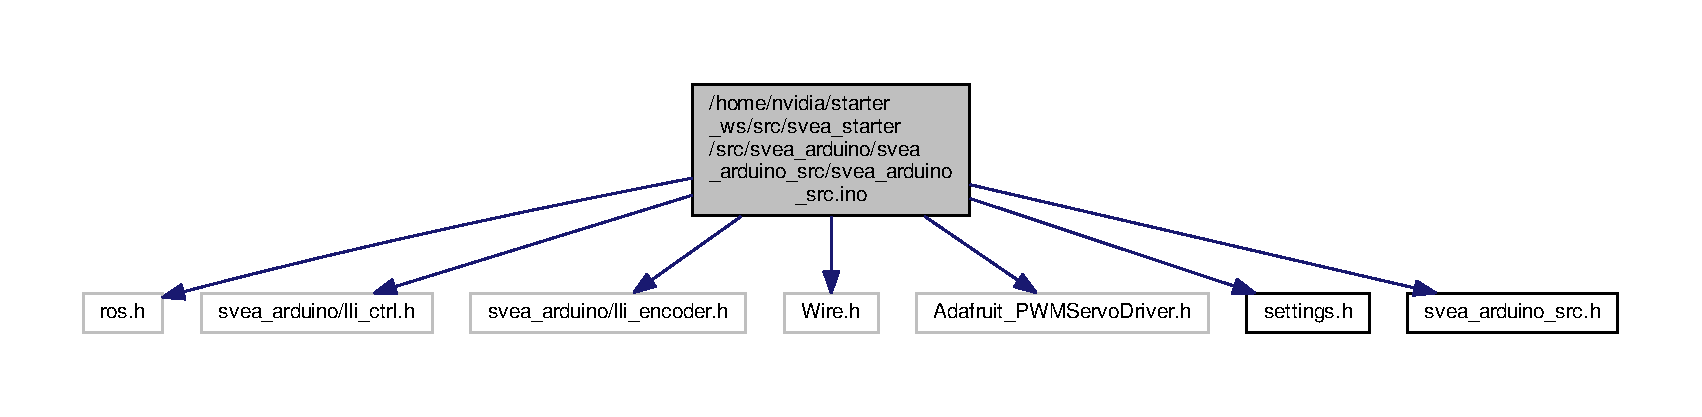
\includegraphics[width=350pt]{svea__arduino__src_8ino__incl}
\end{center}
\end{figure}
\subsection*{Functions}
\begin{DoxyCompactItemize}
\item 
void \hyperlink{svea__arduino__src_8ino_adab070eb39b45b4c79b5d7e3cafa9514}{set\+\_\+pwm\+\_\+driver} (uint8\+\_\+t channel, int8\+\_\+t in\+\_\+value)
\begin{DoxyCompactList}\small\item\em Set actuation P\+WM convert a 8 bit actuation value to a pwm signal and send it to the pwm board. The value gets scaled to a duration that suits the servos (approximately 1 to 2 milli seconds). The scalling uses frequency measurements from pin 10 on the pwm board. \end{DoxyCompactList}\item 
void \hyperlink{svea__arduino__src_8ino_aa5545eb35f187e5fd11a483a265bed7b}{actuate} (const int8\+\_\+t actuation\+\_\+values\mbox{[}$\,$\mbox{]})
\begin{DoxyCompactList}\small\item\em Send settings to the pwm board through \hyperlink{svea__arduino__src_8ino_adab070eb39b45b4c79b5d7e3cafa9514}{set\+\_\+pwm\+\_\+driver()} \end{DoxyCompactList}\item 
uint8\+\_\+t \hyperlink{svea__arduino__src_8ino_ad7d57085af575cbb5dc21e523f3a3321}{set\+\_\+actuated\+\_\+code} ()\hypertarget{svea__arduino__src_8ino_ad7d57085af575cbb5dc21e523f3a3321}{}\label{svea__arduino__src_8ino_ad7d57085af575cbb5dc21e523f3a3321}

\begin{DoxyCompactList}\small\item\em set the control code in messages sent to the computer \end{DoxyCompactList}\item 
void \hyperlink{svea__arduino__src_8ino_ae79b6def446edd5a233efe74bc1f2a7b}{cb\+\_\+ctrl\+\_\+request} (const \hyperlink{svea__arduino__src_8h_a397644608f772ef60685f6a938f43ea1}{lli\+\_\+ctrl\+\_\+in} \&data)
\begin{DoxyCompactList}\small\item\em Callback function for control requests from R\+OS Interprets the message and sends the values to the pwm board through \hyperlink{svea__arduino__src_8ino_aa5545eb35f187e5fd11a483a265bed7b}{actuate()}. \end{DoxyCompactList}\item 
void \hyperlink{svea__arduino__src_8ino_af99fa97e441e842b197dacc4a1a95a99}{process\+Pwm} ()
\begin{DoxyCompactList}\small\item\em Handle pwm events. \end{DoxyCompactList}\item 
void \hyperlink{svea__arduino__src_8ino_a2948125fe6592c36c5c0e641478e2db0}{pwm\+Event} ()\hypertarget{svea__arduino__src_8ino_a2948125fe6592c36c5c0e641478e2db0}{}\label{svea__arduino__src_8ino_a2948125fe6592c36c5c0e641478e2db0}

\begin{DoxyCompactList}\small\item\em Called when a pwm signal from the remote has been recieved Takes the actuation values from the remote and sends them to R\+OS. The frequency of the R\+OS messages is around 100 Hz, based on the frequency of the reciever. If the computer is not sending any signals or the \hyperlink{group__StatusVariables_gae31e17311163c382d2de940091954419}{R\+E\+M\+\_\+\+O\+V\+E\+R\+R\+I\+DE} flag is set (by pushing the deifferential switch to the formost position) the actuation values will also be sent to the pwm board through \hyperlink{svea__arduino__src_8ino_aa5545eb35f187e5fd11a483a265bed7b}{actuate()}. \end{DoxyCompactList}\item 
int8\+\_\+t \hyperlink{svea__arduino__src_8ino_a1c4a5154127fe3f9963eb968b0714b90}{pwm\+\_\+to\+\_\+actuation} (unsigned long duration)
\item 
void \hyperlink{svea__arduino__src_8ino_ab3d64504be0ebfe1754aec5485ddbb72}{tune\+\_\+pwm\+\_\+freq} ()\hypertarget{svea__arduino__src_8ino_ab3d64504be0ebfe1754aec5485ddbb72}{}\label{svea__arduino__src_8ino_ab3d64504be0ebfe1754aec5485ddbb72}

\begin{DoxyCompactList}\small\item\em Tune the frequency of the pwm board Measure the frequency from the pwm board on pin 10 and adjust the frequency to match \hyperlink{group__ActuationToOutput_ga1e7ca795ca78a0b20f4fbc06ea505cfb}{P\+W\+M\+\_\+\+F\+R\+E\+Q\+U\+E\+N\+CY} Will then measure the adjusted value and futher tune \hyperlink{group__ActuationToOutput_gaa6aecad7bb848a436df0b7c89aa1f48f}{P\+W\+M\+\_\+\+N\+E\+U\+T\+R\+A\+L\+\_\+\+T\+I\+CK} and \hyperlink{group__ActuationToOutput_ga8e7323c31db382601e81947c2bba345b}{I\+N\+P\+U\+T\+\_\+\+S\+C\+A\+LE}. If Pin D3 is not connected to pin 10 on the pwm board weirdnes might ensue. \end{DoxyCompactList}\item 
void \hyperlink{svea__arduino__src_8ino_a11eacef653351913656e56d12c152346}{process\+Encoder\+Ticks} ()
\begin{DoxyCompactList}\small\item\em Count the encoder ticks since last call and send the result to R\+OS. \end{DoxyCompactList}\item 
\hyperlink{svea__arduino__src_8ino_afea150fcd685610cb9f7672fce361e53}{I\+SR} (I\+N\+T0\+\_\+vect)
\begin{DoxyCompactList}\small\item\em Interrupt on D2, for detecting rising edges in the pwm signal from the reciever. \end{DoxyCompactList}\item 
\hyperlink{svea__arduino__src_8ino_a22acfb428840c6d9aa212764589cf6c6}{I\+SR} (I\+N\+T1\+\_\+vect)\hypertarget{svea__arduino__src_8ino_a22acfb428840c6d9aa212764589cf6c6}{}\label{svea__arduino__src_8ino_a22acfb428840c6d9aa212764589cf6c6}

\begin{DoxyCompactList}\small\item\em Interrupt on D3, measures frequency of the pwm board. Used for tuning the pwm frequency. D3 should be connected to pin 10 on the pwm board. \end{DoxyCompactList}\item 
\hyperlink{svea__arduino__src_8ino_aa64c6dce15e9de9105b4ae9533c9a267}{I\+SR} (P\+C\+I\+N\+T0\+\_\+vect)\hypertarget{svea__arduino__src_8ino_aa64c6dce15e9de9105b4ae9533c9a267}{}\label{svea__arduino__src_8ino_aa64c6dce15e9de9105b4ae9533c9a267}

\begin{DoxyCompactList}\small\item\em Detects falling edges from the reciever pwm. Interrupt on pins D8 ... D12 (P\+O\+R\+TB) Called on pin change on any reciever channel Store time and the pins that have changed in buffers on falling edges and ignores rising edges. \end{DoxyCompactList}\item 
\hyperlink{svea__arduino__src_8ino_a9c4665742c6b6eb1f0bb9dde41f7cba3}{I\+SR} (P\+C\+I\+N\+T2\+\_\+vect)\hypertarget{svea__arduino__src_8ino_a9c4665742c6b6eb1f0bb9dde41f7cba3}{}\label{svea__arduino__src_8ino_a9c4665742c6b6eb1f0bb9dde41f7cba3}

\begin{DoxyCompactList}\small\item\em Detect ticks from the wheel encoders. Interrupt on pins D0 ... D7 (P\+O\+R\+TD) Called on ticks from eithr encoder. Detects changes in pin values of pin D6 (right wheel) and D7 (left wheel). And increments the tickcounts R\+I\+G\+H\+T\+\_\+\+T\+I\+C\+K\+\_\+\+C\+O\+U\+NT and L\+E\+F\+T\+\_\+\+T\+I\+C\+K\+\_\+\+C\+O\+U\+NT accordingly. \end{DoxyCompactList}\item 
void \hyperlink{svea__arduino__src_8ino_a4fc01d736fe50cf5b977f755b675f11d}{setup} ()\hypertarget{svea__arduino__src_8ino_a4fc01d736fe50cf5b977f755b675f11d}{}\label{svea__arduino__src_8ino_a4fc01d736fe50cf5b977f755b675f11d}

\begin{DoxyCompactList}\small\item\em Arduino setup function. \end{DoxyCompactList}\item 
void \hyperlink{svea__arduino__src_8ino_afe461d27b9c48d5921c00d521181f12f}{loop} ()\hypertarget{svea__arduino__src_8ino_afe461d27b9c48d5921c00d521181f12f}{}\label{svea__arduino__src_8ino_afe461d27b9c48d5921c00d521181f12f}

\begin{DoxyCompactList}\small\item\em Main loop. \end{DoxyCompactList}\end{DoxyCompactItemize}


\subsection{Function Documentation}
\index{svea\+\_\+arduino\+\_\+src.\+ino@{svea\+\_\+arduino\+\_\+src.\+ino}!actuate@{actuate}}
\index{actuate@{actuate}!svea\+\_\+arduino\+\_\+src.\+ino@{svea\+\_\+arduino\+\_\+src.\+ino}}
\subsubsection[{\texorpdfstring{actuate(const int8\+\_\+t actuation\+\_\+values[])}{actuate(const int8_t actuation_values[])}}]{\setlength{\rightskip}{0pt plus 5cm}void actuate (
\begin{DoxyParamCaption}
\item[{const int8\+\_\+t}]{actuation\+\_\+values\mbox{[}$\,$\mbox{]}}
\end{DoxyParamCaption}
)}\hypertarget{svea__arduino__src_8ino_aa5545eb35f187e5fd11a483a265bed7b}{}\label{svea__arduino__src_8ino_aa5545eb35f187e5fd11a483a265bed7b}


Send settings to the pwm board through \hyperlink{svea__arduino__src_8ino_adab070eb39b45b4c79b5d7e3cafa9514}{set\+\_\+pwm\+\_\+driver()} 

\begin{DoxySeeAlso}{See also}
\hyperlink{svea__arduino__src_8ino_adab070eb39b45b4c79b5d7e3cafa9514}{set\+\_\+pwm\+\_\+driver} 
\end{DoxySeeAlso}

\begin{DoxyParams}{Parameters}
{\em actuation\+\_\+values} & array containg 5 values. \\
\hline
\end{DoxyParams}


Definition at line 41 of file svea\+\_\+arduino\+\_\+src.\+ino.

\index{svea\+\_\+arduino\+\_\+src.\+ino@{svea\+\_\+arduino\+\_\+src.\+ino}!cb\+\_\+ctrl\+\_\+request@{cb\+\_\+ctrl\+\_\+request}}
\index{cb\+\_\+ctrl\+\_\+request@{cb\+\_\+ctrl\+\_\+request}!svea\+\_\+arduino\+\_\+src.\+ino@{svea\+\_\+arduino\+\_\+src.\+ino}}
\subsubsection[{\texorpdfstring{cb\+\_\+ctrl\+\_\+request(const lli\+\_\+ctrl\+\_\+in \&data)}{cb_ctrl_request(const lli_ctrl_in &data)}}]{\setlength{\rightskip}{0pt plus 5cm}void cb\+\_\+ctrl\+\_\+request (
\begin{DoxyParamCaption}
\item[{const {\bf lli\+\_\+ctrl\+\_\+in} \&}]{data}
\end{DoxyParamCaption}
)}\hypertarget{svea__arduino__src_8ino_ae79b6def446edd5a233efe74bc1f2a7b}{}\label{svea__arduino__src_8ino_ae79b6def446edd5a233efe74bc1f2a7b}


Callback function for control requests from R\+OS Interprets the message and sends the values to the pwm board through \hyperlink{svea__arduino__src_8ino_aa5545eb35f187e5fd11a483a265bed7b}{actuate()}. 


\begin{DoxyParams}{Parameters}
{\em data} & Message to be evaluated \\
\hline
\end{DoxyParams}


Definition at line 94 of file svea\+\_\+arduino\+\_\+src.\+ino.

\index{svea\+\_\+arduino\+\_\+src.\+ino@{svea\+\_\+arduino\+\_\+src.\+ino}!I\+SR@{I\+SR}}
\index{I\+SR@{I\+SR}!svea\+\_\+arduino\+\_\+src.\+ino@{svea\+\_\+arduino\+\_\+src.\+ino}}
\subsubsection[{\texorpdfstring{I\+S\+R(\+I\+N\+T0\+\_\+vect)}{ISR(INT0_vect)}}]{\setlength{\rightskip}{0pt plus 5cm}I\+SR (
\begin{DoxyParamCaption}
\item[{I\+N\+T0\+\_\+vect}]{}
\end{DoxyParamCaption}
)}\hypertarget{svea__arduino__src_8ino_afea150fcd685610cb9f7672fce361e53}{}\label{svea__arduino__src_8ino_afea150fcd685610cb9f7672fce361e53}


Interrupt on D2, for detecting rising edges in the pwm signal from the reciever. 

Called on rising edge of steering The rising edges of all pwm signals from the reciever are synced, so only one start time is necessary. 

Definition at line 366 of file svea\+\_\+arduino\+\_\+src.\+ino.

\index{svea\+\_\+arduino\+\_\+src.\+ino@{svea\+\_\+arduino\+\_\+src.\+ino}!process\+Encoder\+Ticks@{process\+Encoder\+Ticks}}
\index{process\+Encoder\+Ticks@{process\+Encoder\+Ticks}!svea\+\_\+arduino\+\_\+src.\+ino@{svea\+\_\+arduino\+\_\+src.\+ino}}
\subsubsection[{\texorpdfstring{process\+Encoder\+Ticks()}{processEncoderTicks()}}]{\setlength{\rightskip}{0pt plus 5cm}void process\+Encoder\+Ticks (
\begin{DoxyParamCaption}
{}
\end{DoxyParamCaption}
)}\hypertarget{svea__arduino__src_8ino_a11eacef653351913656e56d12c152346}{}\label{svea__arduino__src_8ino_a11eacef653351913656e56d12c152346}


Count the encoder ticks since last call and send the result to R\+OS. 

The time\+\_\+delta is given in 10 micro seconds resolution. 

Definition at line 331 of file svea\+\_\+arduino\+\_\+src.\+ino.

\index{svea\+\_\+arduino\+\_\+src.\+ino@{svea\+\_\+arduino\+\_\+src.\+ino}!process\+Pwm@{process\+Pwm}}
\index{process\+Pwm@{process\+Pwm}!svea\+\_\+arduino\+\_\+src.\+ino@{svea\+\_\+arduino\+\_\+src.\+ino}}
\subsubsection[{\texorpdfstring{process\+Pwm()}{processPwm()}}]{\setlength{\rightskip}{0pt plus 5cm}void process\+Pwm (
\begin{DoxyParamCaption}
{}
\end{DoxyParamCaption}
)}\hypertarget{svea__arduino__src_8ino_af99fa97e441e842b197dacc4a1a95a99}{}\label{svea__arduino__src_8ino_af99fa97e441e842b197dacc4a1a95a99}


Handle pwm events. 

Reads all the values from \hyperlink{group__PwmMeasurtement_ga1980b7b5ba1ceabb0b5c60c9da70164e}{P\+W\+M\+\_\+\+T\+\_\+\+B\+U\+F\+F\+ER} and \hyperlink{group__PwmMeasurtement_gaed4f8ecf3e1ca2d8bfa8904a43729f57}{P\+W\+M\+\_\+\+S\+\_\+\+B\+U\+F\+F\+ER} that has been added since the last loop and translates the pwm signal to actuation values. Calls \hyperlink{svea__arduino__src_8ino_a2948125fe6592c36c5c0e641478e2db0}{pwm\+Event()} 3 ms after the last observed rising edge.

Button value directions\+: Ctrl / Value Throttle pulled -\/$>$ Possitve value Steering forward -\/$>$ Possitive value Gear switch up -\/$>$ 0 (Low gear) Gear switch down -\/$>$ 1 (High Gear) Switch back -\/$>$ forward diff 0 (unlocked), back diff 0 (unlocked) Switch middle -\/$>$ forward diff 1 (locked), back diff 0 (unlocked) Switch middle -\/$>$ forward diff 1 (locked), back diff 1 (locked) and R\+E\+M\+\_\+\+O\+V\+E\+R\+R\+I\+DE = true 

Definition at line 140 of file svea\+\_\+arduino\+\_\+src.\+ino.

\index{svea\+\_\+arduino\+\_\+src.\+ino@{svea\+\_\+arduino\+\_\+src.\+ino}!pwm\+\_\+to\+\_\+actuation@{pwm\+\_\+to\+\_\+actuation}}
\index{pwm\+\_\+to\+\_\+actuation@{pwm\+\_\+to\+\_\+actuation}!svea\+\_\+arduino\+\_\+src.\+ino@{svea\+\_\+arduino\+\_\+src.\+ino}}
\subsubsection[{\texorpdfstring{pwm\+\_\+to\+\_\+actuation(unsigned long duration)}{pwm_to_actuation(unsigned long duration)}}]{\setlength{\rightskip}{0pt plus 5cm}int8\+\_\+t pwm\+\_\+to\+\_\+actuation (
\begin{DoxyParamCaption}
\item[{unsigned long}]{duration}
\end{DoxyParamCaption}
)}\hypertarget{svea__arduino__src_8ino_a1c4a5154127fe3f9963eb968b0714b90}{}\label{svea__arduino__src_8ino_a1c4a5154127fe3f9963eb968b0714b90}
Convert a pwm duration to an actuation value Usese measurements of pin 10 on the pwm board. \begin{DoxySeeAlso}{See also}
\hyperlink{svea__arduino__src_8ino_ab3d64504be0ebfe1754aec5485ddbb72}{tune\+\_\+pwm\+\_\+freq()} 
\end{DoxySeeAlso}

\begin{DoxyParams}{Parameters}
{\em duration} & Duration of the high part of the pwm signal in micro seconds. \\
\hline
\end{DoxyParams}


Definition at line 266 of file svea\+\_\+arduino\+\_\+src.\+ino.

\index{svea\+\_\+arduino\+\_\+src.\+ino@{svea\+\_\+arduino\+\_\+src.\+ino}!set\+\_\+pwm\+\_\+driver@{set\+\_\+pwm\+\_\+driver}}
\index{set\+\_\+pwm\+\_\+driver@{set\+\_\+pwm\+\_\+driver}!svea\+\_\+arduino\+\_\+src.\+ino@{svea\+\_\+arduino\+\_\+src.\+ino}}
\subsubsection[{\texorpdfstring{set\+\_\+pwm\+\_\+driver(uint8\+\_\+t channel, int8\+\_\+t in\+\_\+value)}{set_pwm_driver(uint8_t channel, int8_t in_value)}}]{\setlength{\rightskip}{0pt plus 5cm}void set\+\_\+pwm\+\_\+driver (
\begin{DoxyParamCaption}
\item[{uint8\+\_\+t}]{channel, }
\item[{int8\+\_\+t}]{in\+\_\+value}
\end{DoxyParamCaption}
)\hspace{0.3cm}{\ttfamily [inline]}}\hypertarget{svea__arduino__src_8ino_adab070eb39b45b4c79b5d7e3cafa9514}{}\label{svea__arduino__src_8ino_adab070eb39b45b4c79b5d7e3cafa9514}


Set actuation P\+WM convert a 8 bit actuation value to a pwm signal and send it to the pwm board. The value gets scaled to a duration that suits the servos (approximately 1 to 2 milli seconds). The scalling uses frequency measurements from pin 10 on the pwm board. 

\begin{DoxySeeAlso}{See also}
\hyperlink{group__ActuationToOutput_ga8e7323c31db382601e81947c2bba345b}{I\+N\+P\+U\+T\+\_\+\+S\+C\+A\+LE} 

\hyperlink{group__ActuationToOutput_gaa6aecad7bb848a436df0b7c89aa1f48f}{P\+W\+M\+\_\+\+N\+E\+U\+T\+R\+A\+L\+\_\+\+T\+I\+CK} To avoid servo jitter at neutral a small dead zone exists around 0. 

\hyperlink{settings_8h_a8f059a42c098816d4ccebaf48add0a4a}{D\+E\+A\+D\+\_\+\+Z\+O\+NE} 
\end{DoxySeeAlso}

\begin{DoxyParams}{Parameters}
{\em channel} & The channel (pin) of the pwm board to send to. \\
\hline
{\em in\+\_\+value} & Value, between -\/127 and 127. to send. \\
\hline
\end{DoxyParams}


Definition at line 27 of file svea\+\_\+arduino\+\_\+src.\+ino.


%--- End generated contents ---

% Index
\backmatter
\newpage
\phantomsection
\clearemptydoublepage
\addcontentsline{toc}{chapter}{Index}
\printindex

\end{document}
